\documentclass[11pt,oneside]{book}

% This project follows the supplied COM dissertation template while extending
% it with packages needed for reproducible tables, figures, and appendices.
\usepackage[utf8]{inputenc}
\usepackage[T1]{fontenc}
\usepackage{lmodern}
\usepackage[a4paper,margin=1.2in]{geometry}
\usepackage{setspace}
\usepackage{graphicx}
\usepackage{booktabs}
\usepackage{tabularx}
\usepackage{longtable}
\usepackage{array}
\usepackage{multirow}
\usepackage{amsmath,amssymb}
\usepackage{microtype}
\usepackage{xcolor}
\usepackage{enumitem}
\usepackage{caption}
\usepackage{subcaption}
\usepackage{float}
\usepackage{url}
\usepackage[numbers,sort&compress]{natbib}
\usepackage[hidelinks]{hyperref}
\usepackage[nameinlink,noabbrev]{cleveref}
\usepackage{fancyhdr}

\definecolor{uosviolet}{RGB}{68,35,89}
\definecolor{accentblue}{RGB}{35,86,122}
\definecolor{softgray}{RGB}{245,245,245}

\newcommand{\thesistitle}{Understanding Failure Modes in Multi-Agent LLM Reasoning Under Controlled Compute Budgets}
\newcommand{\studentname}{Youheng Xie}
\newcommand{\supervisorname}{Robert Loftin}
\newcommand{\degreeprogramme}{MSc Artificial Intelligence}
\newcommand{\submissiondate}{August 2026}
\newcommand{\reportedwordcount}{approximately 12,100 words}

\hypersetup{
  pdftitle={\thesistitle},
  pdfauthor={\studentname},
  pdfsubject={COM Dissertation},
  pdfkeywords={large language models, multi-agent systems, multi-hop question answering, human audit, failure localisation}
}

\setstretch{1.35}
\setlength{\parindent}{1.5em}
\setlength{\parskip}{0.15em}
\setlength{\emergencystretch}{2em}
\setcounter{secnumdepth}{3}
\setcounter{tocdepth}{2}
\captionsetup{font=small,labelfont=bf}
\renewcommand{\arraystretch}{1.15}

\pagestyle{fancy}
\fancyhf{}
\fancyhead[L]{\small\nouppercase{\leftmark}}
\fancyhead[R]{\small\thepage}
\renewcommand{\headrulewidth}{0.4pt}
\fancypagestyle{plain}{
  \fancyhf{}
  \fancyfoot[C]{\thepage}
  \renewcommand{\headrulewidth}{0pt}
}

\newcommand{\correct}{\ensuremath{\mathrm{C}}}
\newcommand{\wrong}{\ensuremath{\mathrm{W}}}
\newcommand{\uncertain}{\ensuremath{\mathrm{U}}}
\newcommand{\ctow}{\ensuremath{\correct\!\rightarrow\!\wrong}}
\newcommand{\wtoc}{\ensuremath{\wrong\!\rightarrow\!\correct}}
\newcommand{\sas}{\textsc{SAS}}
\newcommand{\mas}{\textsc{MAS}}

\begin{document}
\hypersetup{pageanchor=false}

\begin{titlepage}
  \centering
  
\includegraphics[width=0.33\textwidth]{images/UOSLogo_Portrait_Violet_RGB.png}\par
  \vspace{1.4cm}
  {\Huge\bfseries\color{uosviolet}\thesistitle\par}
  \vspace{1.3cm}
  {\Large\studentname\par}
  \vspace{0.7cm}
  {\large A dissertation submitted in partial fulfilment of the requirements for the degree of\par}
  \vspace{0.4cm}
  {\Large\bfseries\degreeprogramme\par}
  \vfill
  {\large School of Computer Science\par}
  {\large University of Sheffield\par}
  \vspace{0.8cm}
  {\large Supervisor: \supervisorname\par}
  {\large \submissiondate\par}
  \vspace{0.8cm}
  {\small Reported word count: \reportedwordcount\par}
\end{titlepage}

\frontmatter
\hypersetup{pageanchor=true}

\chapter*{Declaration}
\addcontentsline{toc}{chapter}{Declaration}
All sentences or passages quoted in this dissertation from other people's work have been specifically acknowledged by clear cross-referencing to author, work and page(s). Any illustrations that are not the work of the author of this dissertation have been used with the explicit permission of the originator and are specifically acknowledged. I understand that failure to do this amounts to plagiarism and will be considered grounds for failure in this dissertation and the degree examination as a whole.

\vspace{1.5cm}
\noindent Signed: \rule{0.45\textwidth}{0.4pt}\hfill Date: \rule{0.22\textwidth}{0.4pt}

\chapter*{Acknowledgements}
\addcontentsline{toc}{chapter}{Acknowledgements}
I thank my supervisor, \supervisorname, for guidance on the framing, evaluation design, and interpretation of this project. I also acknowledge the University of Sheffield research computing facilities used to run the experiments. Any remaining errors are my own.

\chapter*{Abstract}
\addcontentsline{toc}{chapter}{Abstract}

Multi-agent language-model systems are often justified by an intuitive division-of-labour argument: several agents can explore more candidate answers than one agent, after which communication and aggregation should select the best result. Final-answer accuracy alone cannot test this mechanism. It conflates failure to discover the answer with failure to retain, endorse, or select an answer that was already present. This dissertation therefore evaluates multi-agent reasoning as a sequence of state transitions from answer discovery to final endorsement.

The study analyses Qwen3-4B in a frozen form and after supervised fine-tuning on MuSiQue and 2WikiMultiHopQA. A single-agent baseline is compared with five multi-agent architectures under matched thinking-token budgets of 1,000 and 2,000 tokens. The primary benchmark contains 9,600 item-configurations, including 8,000 multi-agent configurations and 26,873 intermediate stages. Lexical accuracy is supplemented by a stage-level semantic screen and a preregistered-style blind human audit focused on the two clearest temporal architectures, Debate and Sequential. The audit covers 160 sampled items, 400 non-repeat stage records, and 20 hidden repeats. It separates whether a stage contains sufficient support for the reference answer (Discovery) from whether the stage commits to that answer (Endorsement).

The principal result is that exploration and decision quality separate. Multi-agent systems often expose a correct answer in at least one intermediate output, but later revision, communication, and aggregation can erase that advantage. In the human audit, the weighted harmful transition rate from a correct source endorsement to a wrong final endorsement was 5.45\% for Debate and 0.59\% for Sequential, a difference of 4.86 percentage points. Conversely, beneficial wrong-to-correct transitions were 0.00\% for Debate and 5.82\% for Sequential. A calibrated Mistral judge agreed with human stage labels at 82.5\% for Discovery and 80.5\% for Endorsement, but targeted transition reliability was too weak for it to serve as ground truth. Machine labels are consequently used only for full-trace screening, while the human audit supports the central transition claims.

Increasing the nominal thinking budget also failed to improve aggregate semantic outcomes: discovery fell from 84.19\% to 82.84\%, final accuracy fell from 74.08\% to 72.82\%, and mean wall time increased by 4.83 seconds per item. These results show that additional computation is not equivalent to useful reasoning when architectures repeatedly regenerate, revise, or compress information. The dissertation contributes an auditable evaluation framework, architecture-specific failure localisation, and evidence that multi-agent reasoning should be assessed by both candidate generation and answer preservation rather than final accuracy alone.


\tableofcontents
\listoffigures
\listoftables

\chapter*{Abbreviations}
\addcontentsline{toc}{chapter}{Abbreviations}
\begin{tabular}{@{}ll@{}}
LLM & Large language model \\
MAS & Multi-agent system \\
SAS & Single-agent system \\
QA & Question answering \\
SFT & Supervised fine-tuning \\
CI & Confidence interval \\
OR & Odds ratio \\
\end{tabular}

\mainmatter
\chapter{Introduction}
\label{chap:introduction}

\section{Motivation}

Large language models (LLMs) can solve many reasoning tasks through a single generated chain of thought, but an increasingly common alternative is to organise several model calls as a multi-agent system (MAS). One agent may decompose a question, several agents may work on subproblems or adopt different roles, and a final component may revise or aggregate their outputs. This design is attractive because it resembles familiar forms of collaborative problem solving. Independent proposals may increase coverage, debate may expose errors, and a dedicated aggregator may separate exploration from decision making. Frameworks such as AutoGen have made these structures straightforward to implement, while work on multi-agent debate reports gains in factuality and reasoning under some settings \citep{wu2023autogen,du2023debate,liang2023mad}.

The same decomposition also introduces new failure surfaces. A correct answer may be present in an early proposal but removed during revision. A final picker may prefer a polished but incorrect alternative. A sequential worker may correctly resolve a subproblem and then lose the answer when new context is appended. An aggregator may ignore a correct candidate in favour of a majority of correlated errors. These are not failures of initial answer discovery. They are failures of preservation, endorsement, and selection. A final exact-match score cannot distinguish them from cases in which no component ever produced useful evidence.

This distinction matters for both scientific and engineering reasons. Scientifically, claims that ``agents reason better together'' concern a mechanism, not only an endpoint. If several agents discover more correct candidates but the system cannot preserve them, the architecture has generated information without converting it into a reliable decision. Engineering decisions are also different under these two diagnoses. A discovery problem may call for better retrieval, more diverse prompts, or a stronger base model. A preservation problem instead calls for provenance-aware aggregation, protected evidence, calibrated confidence, or a less destructive revision policy. Treating both as final-answer error hides the intervention point.

Compute matching creates a second difficulty. A multi-agent graph naturally uses more model invocations than a single-agent baseline. Comparing systems without controlling computation can therefore reward the architecture that simply spends more. Conversely, assigning the same nominal token budget does not guarantee equal effective reasoning: agents can repeat context, emit boilerplate, terminate early, or spend tokens reconciling redundant outputs. Recent work by \citet{tran2026single} directly challenges the assumption that multi-agent decomposition improves multi-hop reasoning when thinking-token budgets are matched. The present dissertation reproduces that comparison with an open 4-billion-parameter model and extends it from outcome measurement to failure localisation.

\section{Problem statement}

The central problem is to determine what happens between the first appearance of a defensible answer and the system's final commitment. In this dissertation, an intermediate output is evaluated along two separate axes. \emph{Discovery} asks whether the output contains enough content to support the reference answer, even when the answer is embedded in a longer discussion. \emph{Endorsement} asks whether the output itself commits to that answer rather than merely mentioning it as one possibility. This separation is necessary because a debate transcript may contain the gold answer while explicitly rejecting it, and an aggregator may copy relevant evidence yet conclude with the wrong entity.

Let the source state be the last architecture-specific point at which the system has a meaningful opportunity to preserve a correct answer. For Debate this is the oracle over the two revised candidates; for Sequential it is the final worker output. The target is the final picker or aggregator. A harmful transition occurs when the source endorses the correct answer and the target endorses a wrong answer (\ctow). A beneficial transition occurs when the source is wrong and the target becomes correct (\wtoc). These transition rates provide a direct measure of the value or damage added by the final coordination operation.

Automated semantic judges make this analysis scalable, but their errors can be especially consequential in deliberately difficult transition strata. A judge that is accurate on ordinary correct and incorrect answers may still confuse mention with endorsement, over-credit partial evidence, or behave inconsistently on truncated outputs. The project therefore adopts a hierarchy of evidence. Lexical metrics provide reproducible benchmark-level outcomes. A calibrated Mistral judge supplies a screen over all recorded stages. A blind human audit is the primary basis for the most important Debate and Sequential transition claims. This hierarchy prevents the scale of machine annotation from being mistaken for validity.

\section{Research questions}

The study addresses three research questions.

\begin{description}[leftmargin=1.5cm,style=nextline]
  \item[RQ1] Under matched thinking-token budgets, how do single-agent and multi-agent architectures differ in final-answer performance, answer discovery, and answer preservation on multi-hop question answering?
  \item[RQ2] When a correct answer is available before the final decision, where do Debate and Sequential architectures lose or recover it, and are these transitions supported by human annotation?
  \item[RQ3] Do larger nominal thinking budgets and higher observed resource use improve semantic outcomes, or can additional computation coincide with lower discovery and higher post-discovery loss?
\end{description}

The questions deliberately move from broad comparison to causal diagnosis without claiming a causal experiment where none exists. RQ1 is a benchmark comparison. RQ2 localises state changes at known architecture boundaries. RQ3 combines matched-budget tests with observational resource associations; the latter are interpreted as descriptive rather than causal.

\section{Contributions}

This dissertation makes five contributions.

\begin{enumerate}[leftmargin=*]
  \item It implements a controlled comparison of a single-agent baseline and five multi-agent architectures -- Sequential, Subtask Parallel, Parallel Roles, Debate, and Ensemble -- using the same Qwen3-4B base family, fixed evaluation subsets, and matched nominal thinking-token budgets.
  \item It reframes multi-agent performance as a transition process. Discovery, oracle availability, preservation, aggregation regret, and final endorsement are measured separately, making it possible to distinguish generation failures from coordination failures.
  \item It develops a blind audit protocol that labels both Discovery and Endorsement, includes hidden repeated records for intra-rater consistency, freezes the sampling strata before unblinding, and reports finite-population weighted estimates for the target benchmark population.
  \item It shows an architecture-specific asymmetry in the audited data. Debate's final decision is predominantly destructive: the weighted harmful \ctow{} rate is 5.45\% and the beneficial \wtoc{} rate is 0.00\%. Sequential aggregation is less often harmful and sometimes corrective: 0.59\% harmful and 5.82\% beneficial.
  \item It demonstrates that nominally larger budgets are not automatically useful. Across 4,000 matched multi-agent pairs, moving from 1,000 to 2,000 thinking tokens increases mean wall time by 4.83 seconds while reducing both semantic discovery and final semantic accuracy.
\end{enumerate}

The numerical contributions should be read with their stated scope. The human audit supports population-weighted claims for the frozen sampling frame used to construct the audit. The full 26,873-stage semantic analysis is valuable for locating candidate failure mechanisms, but the Mistral labels do not meet the reliability standard required to convert every screened transition into ground truth.

\section{Dissertation structure}

\Cref{chap:related} positions the work in research on multi-agent reasoning, multi-hop QA, process evaluation, and automated judging. \Cref{chap:framework} defines the state-transition framework and the metrics used throughout. \Cref{chap:design} describes models, datasets, architectures, budgets, and the execution protocol, while \Cref{chap:evaluation} explains lexical scoring, semantic screening, calibration, blind human annotation, and statistical analysis. The results then follow the progression of the research. \Cref{chap:benchmark-results} first reports the matched-budget benchmark, the completed fine-tuning intervention, and the budget comparison. \Cref{chap:machine-results} asks why the outcome pattern occurs by using the full-trace Mistral screen to examine discovery, preservation, and failure location. \Cref{chap:human-results} evaluates judge reliability and reports the human-audited transition estimates. \Cref{chap:discussion} interprets the combined evidence and derives design implications. \Cref{chap:limitations} bounds the claims, and \Cref{chap:conclusion} answers the research questions and identifies the most defensible next steps.

\chapter{Related Work}
\label{chap:related}

\section{Reasoning with a single language model}

Modern language-model reasoning systems often begin with chain-of-thought prompting, which elicits intermediate natural-language steps before an answer \citep{wei2022chain}. The important methodological insight is that reasoning quality depends not only on the final string but on the trajectory that produces it. Self-consistency extends this idea by sampling multiple reasoning paths and selecting the most consistent answer, thereby separating candidate generation from aggregation without requiring persistent agent identities \citep{wang2023selfconsistency}. Iterative approaches such as Self-Refine and Reflexion add feedback and revision loops to a single model \citep{madaan2023selfrefine,shinn2023reflexion}. These methods demonstrate that repeated computation can help, but they also expose a general risk shared with multi-agent systems: later text can overwrite a correct earlier state.

This dissertation uses a single-agent system (SAS) as the primary baseline because architecture comparisons are only meaningful relative to a strong, compute-aware alternative. A weak one-shot baseline would confound decomposition with additional inference. The SAS receives the same question and oracle context as the multi-agent systems and is evaluated at the same nominal thinking-token levels. This follows the matched-compute emphasis of \citet{tran2026single}, who argue that the apparent benefit of multi-agent reasoning can diminish or reverse once the comparison controls for thinking tokens.

Single-agent self-consistency is related to the Ensemble architecture studied here, but the decision rules differ. Self-consistency normally aggregates answers by agreement, while this implementation exposes several candidate generations to a final language-model aggregator. The latter can in principle use evidence quality rather than frequency, but it can also introduce selection error. This distinction motivates the oracle-final gap used later: the gap measures how often an answer was available among candidates but was not converted into a correct final prediction.

\section{Multi-agent language-model systems}

Multi-agent LLM systems distribute inference across interacting calls that are described as agents. The term covers substantially different computational graphs. Some systems use independent roles to diversify viewpoints, some use planners and workers to decompose tasks, and others use adversarial critique. AutoGen provides a general conversation-based framework in which specialised agents exchange messages and invoke tools \citep{wu2023autogen}. Such flexibility is useful for applications, but it makes scientific comparison difficult: changing the number of calls, prompts, stopping conditions, and aggregation logic can change both compute and behaviour.

Multi-agent debate is one prominent family. \citet{du2023debate} report that multiple model instances proposing and debating answers can improve factuality and reasoning. \citet{liang2023mad} similarly motivate debate as a mechanism for divergent thinking and mitigation of degenerate consensus. At a high level, debate has two expected benefits. First, independent proposals increase the probability that at least one agent finds a correct answer. Second, revision after observing another proposal may correct mistakes. However, debate also adds two decision points: revisions may turn correct proposals into wrong ones, and a final picker may choose the wrong revised answer. The present study measures both points rather than treating debate as a single black box.

Planner-worker architectures make a different promise. A planner decomposes a multi-hop question into subquestions; workers solve these steps either sequentially or in parallel; and an aggregator forms the final answer. Sequential execution can propagate useful evidence from one worker to the next, but later workers inherit earlier errors and may displace previously correct content. Parallel execution reduces error propagation and latency but deprives workers of intermediate findings. Role-based parallelism seeks diversity by asking several agents to analyse the same evidence from different perspectives. An ensemble samples multiple answers with stochastic decoding. These architectures should not be treated as interchangeable instances of ``more agents'' because they create different source states and different opportunities for loss.

The dissertation therefore treats architecture as a temporal data-generating process. Debate is proposal $\rightarrow$ revision $\rightarrow$ picker. Sequential is plan $\rightarrow$ worker chain $\rightarrow$ aggregator. Parallel Roles and Ensemble are candidate set $\rightarrow$ aggregator. Subtask Parallel is plan $\rightarrow$ partial findings $\rightarrow$ aggregator. The source-stage semantics differ: a subtask finding is not necessarily expected to answer the full question, whereas a revised debate answer is. This is why the strongest human transition comparison is restricted to Debate and Sequential, where the source and target states are interpretable and the final boundary is explicit.

\section{Multi-hop question answering}

Multi-hop QA is a natural test bed for decomposition because the answer is intended to require combining facts. MuSiQue was constructed by composing single-hop questions while applying filters designed to reduce shortcut solutions \citep{trivedi2022musique}. 2WikiMultiHopQA provides questions requiring reasoning over evidence from multiple Wikipedia pages and includes supporting facts intended to expose reasoning steps \citep{ho2020twowiki}. The datasets differ in difficulty and construction, which makes their joint use valuable: an architectural pattern that appears on only one dataset may reflect dataset-specific answer forms or shortcut opportunities.

At the same time, benchmark labels do not prove that a model used the intended reasoning chain. \citet{min2019compositional} showed that compositional questions can often be answered without the expected multi-hop process. For this reason, the present dissertation does not claim to verify latent reasoning. It evaluates observable text states: whether an answer-equivalent claim appears, whether the system endorses it, and whether later components preserve it. Oracle context is supplied so that the experiment focuses on reasoning and coordination rather than retrieval. This narrows the claim but improves internal interpretability: absence of the answer cannot be attributed to a failed document retriever.

Exact match and token-level F1 remain useful because they are transparent and reproducible, but they are brittle for semantically equivalent answers. An output may include the correct entity with explanatory text, an alias, a date format, or a harmless modifier and still fail strict matching. Conversely, substring matching can over-credit an answer mentioned only to reject it. These limitations are amplified at intermediate stages, whose outputs are not written in final-answer format. The project consequently reports lexical final accuracy for continuity with standard QA evaluation and uses a separate semantic protocol for stage localisation.

\section{Process evaluation and failure localisation}

Outcome supervision assigns a label to a completed response. Process supervision evaluates intermediate steps, potentially detecting where an otherwise promising trajectory goes wrong. Work such as \citet{lightman2023verify} demonstrates the value of step-level feedback for mathematical reasoning. The setting here is related but not identical. Intermediate stages are not individual mathematical derivations; they are messages produced by different architectural roles. A useful label must therefore be role-aware and must distinguish informational presence from the system's decision.

The dissertation introduces two observable variables for every relevant stage. Discovery records whether the reference answer is substantively available in the text. Endorsement records whether the text's answer-bearing statement commits to it. Consider a revised debate output stating that ``Paris is plausible, but the evidence instead supports Lyon.'' Paris has been mentioned but is not endorsed. A presence-only judge may call this correct even though the revision would direct a final picker towards Lyon. Conversely, a worker may provide the exact supporting relationship without formatting a final answer; this can count as discovery even when endorsement is not applicable or remains uncertain. Explicit decision rules are therefore necessary for reproducible transition labels.

The closest quantitative concept is oracle accuracy over a candidate set. If any candidate is correct, an oracle selector would succeed. The difference between oracle and final accuracy is often described as aggregation regret. This project extends the idea temporally. It asks not only whether a correct candidate exists, but whether it survives revision, worker propagation, and final selection. Harmful and beneficial transitions then measure the net behaviour of a coordination step, rather than assuming that aggregation is beneficial whenever candidate coverage is high.

\section{Language models as evaluators}

LLM-based evaluation can approximate human preferences and semantic judgements at a scale that manual annotation cannot match. MT-Bench and Chatbot Arena helped establish the practical use of strong models as judges while documenting biases such as position sensitivity and self-preference \citep{zheng2023judge}. G-Eval uses structured criteria and chain-of-thought evaluation to improve alignment with human judgements on generation tasks \citep{liu2023geval}. These results support machine-assisted evaluation, but they do not justify assuming validity on a new label definition or a deliberately difficult subpopulation.

Reliability is especially important for transition analysis. Suppose a source stage is falsely marked correct and the destination is correctly marked wrong. The resulting \ctow{} transition is entirely artificial. Two individually plausible labels can also form the wrong transition class when one error occurs. General calibration accuracy therefore does not guarantee transition-level accuracy. The present project first calibrated a Mistral judge on ordinary evidence-validity examples, then conducted a targeted human audit on transition-enriched strata. The targeted result was materially worse than the general result, so the dissertation does not use the machine judge as the primary estimator for Debate and Sequential transitions.

Cohen's kappa is reported alongside exact agreement because it adjusts for chance agreement under the observed marginal distributions \citep{cohen1960coefficient}. Bootstrap confidence intervals describe uncertainty in agreement estimates \citep{efron1994bootstrap}. Neither statistic establishes construct validity by itself. Hidden repeats measure one annotator's internal consistency, not independent inter-annotator agreement, and high consistency would not correct a systematically wrong codebook. The audit is therefore designed around explicit evidence checks, blind identifiers, frozen strata, and unblinding only after labels are complete.

\section{Positioning of this dissertation}

Existing work provides strong reasons to test both the promise and the cost of multi-agent decomposition. Debate and ensemble methods motivate diverse candidate generation; matched-compute studies question whether that diversity is worth its inference cost; process evaluation motivates inspection of intermediate states; and LLM-as-judge research offers scale with known validity risks. The gap is a controlled, architecture-aware analysis connecting these strands. This dissertation fills that gap by comparing multiple architectures under common budgets, measuring discovery and final correctness separately, localising loss at specific boundaries, and using human labels to support the claims for which machine errors would be most damaging.

\chapter{Research Questions and Analytical Framework}
\label{chap:framework}

\section{From a final prediction to a state trajectory}

For item $i$, let an architecture produce a sequence of observable stage texts
\begin{equation}
  T_i = \left(s_{i1}, s_{i2}, \ldots, s_{ik}, f_i\right),
\end{equation}
where $f_i$ is the final output and the preceding stages depend on the architecture. Each stage is mapped to two labels: discovery $D(s) \in \{\correct,\wrong,\uncertain\}$ and endorsement $E(s) \in \{\correct,\wrong,\uncertain\}$. The labels are defined relative to the reference answer and accepted aliases.

Discovery is \correct{} when the stage contains an answer-equivalent statement or enough explicit relational content to identify the answer. It is \wrong{} when this support is absent or supports a different answer. Endorsement is \correct{} when the answer-bearing statement commits to the reference answer, and \wrong{} when it commits elsewhere or explicitly rejects the reference answer. \uncertain{} is reserved for genuinely unresolvable cases, principally truncation inside the answer-bearing statement. The distinction is asymmetric: endorsement implies an answer decision, while discovery may be present in text that does not make a final commitment.

\begin{figure}[htbp]
  \centering
  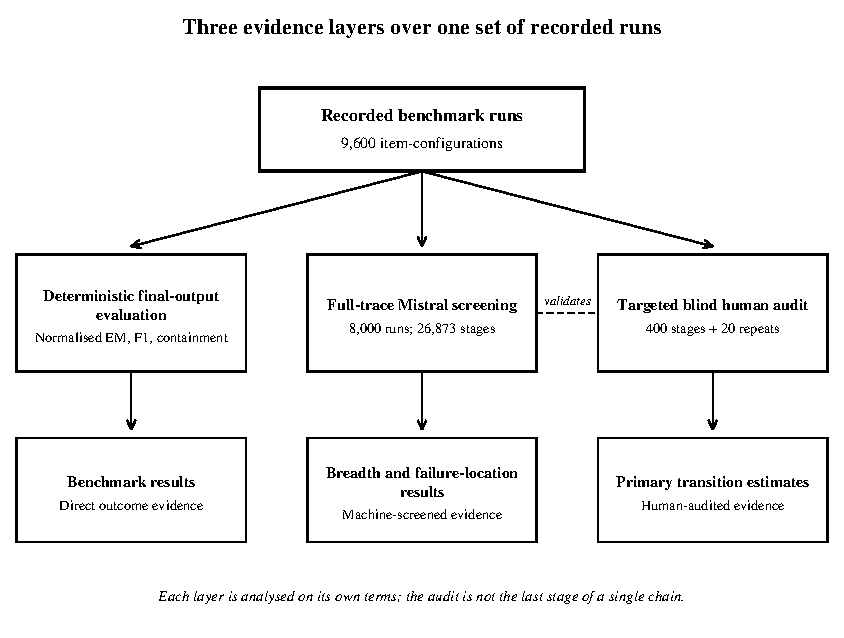
\includegraphics[width=0.96\textwidth]{figures/analysis_pipeline.pdf}
  \caption[Three evidence layers over the recorded runs]{Three evidence layers derived from the recorded benchmark runs. Deterministic final-output evaluation produces benchmark results; full-trace machine labels support breadth screening; and the blind human audit validates selected labels while independently supporting the primary Debate and Sequential transition estimates.}
  \label{fig:pipeline}
\end{figure}

\Cref{fig:pipeline} summarises three evidence layers derived from the recorded runs. Deterministic final-output evaluation produces benchmark results. Full-trace Mistral screening independently produces breadth and failure-location results. The targeted blind human audit both validates selected machine labels and supplies the primary transition estimates. The audit is therefore not merely the last transformation in a single scoring pipeline.

\section{Architecture-specific source states}

A universal definition of ``the previous stage'' would obscure the semantics of different computational graphs. Source states are therefore defined by the last point before the final coordination decision at which correctness can be meaningfully preserved.

For Debate, two agents first produce proposals and then revised answers after exposure to the opposing position. Let $r_{iA}$ and $r_{iB}$ be the revised outputs. The source endorsement is an oracle over these revisions:
\begin{equation}
  E_i^{\mathrm{src}} = \max\left(E(r_{iA}), E(r_{iB})\right),
\end{equation}
where the ordering is $\correct > \uncertain > \wrong$ for availability. The target is the final picker. This boundary measures whether the picker converts a correct revised option into the final answer. A separate machine-screened analysis examines proposal-to-revision changes, but the primary human transition estimate concerns the revision oracle to picker boundary.

For Sequential, workers receive the accumulated state in order. The source is the last worker output and the target is the final aggregator. This captures whether the aggregator preserves the chain's final answer state. Earlier worker transitions are useful diagnostics but are harder to interpret as homogeneous trials because workers may be assigned different subquestions.

For Parallel Roles and Ensemble, the natural source is the oracle over the candidate set and the target is the aggregator. For Subtask Parallel, candidate outputs are partial findings rather than complete answers, so oracle accuracy is not directly comparable with full-answer candidates. These three architectures remain in the benchmark and semantic screen, but are not included in the primary human transition audit.

\section{Outcome and transition metrics}

Final lexical performance is scored against the benchmark's own gold answer and its supplied aliases. The normalisation removes articles, punctuation, and redundant whitespace before comparison. Three comparison rules are used and are kept distinct throughout: normalised exact match, token-level F1, and normalised containment. \Cref{sec:lexical} defines all three formally and \Cref{tab:scoring-examples} gives worked examples of predictions that do and do not match under each. The headline benchmark figures in \Cref{chap:benchmark-results} use normalised containment and are named \emph{final normalised accuracy} there. Semantic metrics use the stage labels defined above.

For $N$ evaluated items, semantic discovery rate is
\begin{equation}
  \mathrm{DiscoveryRate} = \frac{1}{N}\sum_{i=1}^{N} \mathbb{I}\left[\exists s \in T_i : D(s)=\correct\right].
\end{equation}
Candidate-oracle accuracy restricts the maximum to the architecture's designated candidate stages. Final semantic accuracy is the proportion for which $D(f_i)=\correct$ under the screening protocol. Among items with a correct discovered state, preservation rate is
\begin{equation}
  \mathrm{Preservation} = P\left(D(f_i)=\correct \mid \exists s \in T_i : D(s)=\correct\right),
\end{equation}
and drop rate is its complement. Aggregation regret measures the difference between what the candidate set made available and what the system finally delivered,
\begin{equation}
  \mathrm{Regret} = \mathrm{OracleAccuracy} - \mathrm{FinalAccuracy},
  \label{eq:regret}
\end{equation}
where $\mathrm{OracleAccuracy}$ is the candidate-oracle accuracy defined above and $\mathrm{FinalAccuracy}$ is final semantic accuracy, both computed over the same $N$ items. A positive value indicates that the final decision failed to exploit available candidates. A negative value can occur for architectures such as Sequential or Subtask Parallel when aggregation synthesises partial evidence not individually sufficient for an oracle candidate label.

For the human analysis, the primary harmful and beneficial transition indicators are
\begin{align}
  H_i &= \mathbb{I}\left[E_i^{\mathrm{src}}=\correct \land E_i^{\mathrm{final}}=\wrong\right],\\
  B_i &= \mathbb{I}\left[E_i^{\mathrm{src}}=\wrong \land E_i^{\mathrm{final}}=\correct\right].
\end{align}
The rates $P(H_i=1)$ and $P(B_i=1)$ quantify damage and recovery at the final coordination boundary. Reporting both prevents a system with many destructive and many corrective changes from appearing equivalent to a stable system.

\section{Weighting the human audit}

The audit deliberately oversamples transitions that are rare in the full machine-screened population. Raw sample proportions therefore do not estimate population prevalence. Let $h$ index the frozen sampling strata, $N_h$ be the number of eligible items in a stratum, $n_h$ the audited sample, and $\bar{y}_h$ the audited transition rate. The finite-population weighted estimate is
\begin{equation}
  \hat{p} = \sum_h W_h\bar{y}_h, \qquad W_h = \frac{N_h}{\sum_h N_h}.
  \label{eq:weighting}
\end{equation}
An approximate stratified variance is
\begin{equation}
  \widehat{\mathrm{Var}}(\hat{p}) = \sum_h W_h^2\left(1-\frac{n_h}{N_h}\right)\frac{s_h^2}{n_h},
\end{equation}
where $s_h^2$ is the within-stratum sample variance. Intervals use $\hat{p} \pm 1.96\sqrt{\widehat{\mathrm{Var}}(\hat{p})}$ with bounds clipped to $[0,1]$. Because the final within-stratum selection also pursued coverage and balance, these intervals are descriptive approximations rather than confirmatory probability-sample intervals. The weighted point estimates are the primary summaries.

\section{Reliability thresholds and evidence hierarchy}

The project distinguishes three levels of evidence.

\begin{enumerate}[leftmargin=*]
  \item \textbf{Direct benchmark evidence}: exact match, F1, token use, truncation flags, and wall time are computed deterministically from recorded outputs and traces.
  \item \textbf{Machine-screened semantic evidence}: a Mistral judge labels all relevant stages. These data support broad patterns, candidate selection for audit, and descriptive failure localisation.
  \item \textbf{Human-audited transition evidence}: blinded human labels, hidden repeats, and frozen weights support the primary Debate and Sequential transition rates.
\end{enumerate}

This hierarchy follows from observed transfer failure. The judge performed strongly on a broad calibration set but materially worse on difficult transition-enriched examples. A second, stronger Qwen2.5-72B judge improved agreement but still failed the predetermined acceptance thresholds. Rather than selecting whichever machine result best supports a narrative, the analysis retains the human audit as controlling evidence and presents machine outputs with explicit caveats.

\section{Interpretive hypotheses}

The framework yields testable expectations without requiring a single global claim that MAS is good or bad. Architectures with independent candidates should have high discovery and oracle coverage. If their final accuracy is lower, the gap points to aggregation rather than exploration. Debate should show beneficial proposal-to-revision changes if cross-critique works as intended, but harmful changes if social conformity or persuasive errors dominate. Sequential workers should be vulnerable to state loss across the chain, while the final aggregator may recover from incomplete worker formulations. Larger budgets should improve outcomes if additional reasoning is productive; if they instead lengthen outputs, repeat information, or increase revision opportunities, discovery and preservation may stagnate or decline.

These hypotheses structure the results chapter. They are not all evaluated with the same evidential strength. Full-trace patterns generate architecture-level diagnoses, whereas the audited final-boundary estimates determine the main claim about Debate and Sequential preservation.

\chapter{Experimental Design}
\label{chap:design}

\section{Overview}

The experiment is a factorial comparison over dataset, model variant, architecture, and nominal thinking-token budget. Two multi-hop QA datasets are used: MuSiQue and 2WikiMultiHopQA. Two model variants are evaluated: the frozen Qwen3-4B checkpoint and a project fine-tuned variant labelled \texttt{v3b}. Six systems are compared: one single-agent baseline and five multi-agent architectures. Each system is run at budgets of 1,000 and 2,000 thinking tokens on fixed 200-item validation subsets per dataset. Temperature is zero except for the explicitly stochastic candidate generation used by Ensemble.

The complete benchmark therefore contains
\begin{equation}
  2\ \text{datasets} \times 2\ \text{models} \times 6\ \text{systems} \times 2\ \text{budgets} \times 200\ \text{items} = 9{,}600
\end{equation}
item-configurations. Removing the single-agent baseline leaves 8,000 MAS configurations, from which 26,873 intermediate stage outputs are available for semantic screening. The design uses the validation split and a fixed random seed of zero. Oracle context is supplied for each question, so retrieval quality is held outside the scope of the comparison.

\subsection{Units, keys, and data hierarchy}

A \emph{benchmark question} is identified by dataset and the dataset's original question identifier. An \emph{experimental condition} is one dataset $\times$ model variant $\times$ system $\times$ budget combination; there are 48 such conditions. An \emph{item-configuration} is one benchmark question executed under one condition and the fixed seed. Its complete recorded execution is a \emph{trace}. A \emph{stage record} is one observable architecture-level text associated with a named role or saved output position; it is not an individual latent reasoning step or a token. A \emph{repeat} is a blinded duplicate of an existing stage record used only for intra-rater quality control, not a new question, run, or stage.

The 9,600 total therefore count item-configurations, not distinct questions or stages: 1,600 belong to SAS and 8,000 to the five MAS architectures. Different architectures expose different numbers of stage records, which is why the MAS traces contain 26,873 screened intermediate stages rather than a constant multiple of 8,000. Within an SAS raw record, pre-final \path{trace.thinking} and the returned \path{prediction} originate from the same invocation but are stored as distinguishable observable texts. They would form the source and final records in a future architecture-neutral process audit.

\begin{table}[htbp]
  \centering
  \caption[Factorial benchmark design]{Factorial benchmark design.}
  \label{tab:design}
  \begin{tabularx}{\textwidth}{@{}lX@{}}
    \toprule
    Factor & Levels and implementation \\
    \midrule
    Dataset & MuSiQue and 2WikiMultiHopQA; 200 validation items each \\
    Model & Qwen3-4B frozen; Qwen3-4B SFT checkpoint \texttt{v3b} \\
    System & SAS, Sequential, Subtask Parallel, Parallel Roles, Debate, Ensemble \\
    Budget & 1,000 and 2,000 nominal thinking tokens \\
    Context & Oracle evidence passages supplied to every system \\
    Decoding & Temperature 0.0, except Ensemble candidates at temperature 0.7 \\
    Seed & 0 \\
    \bottomrule
  \end{tabularx}
\end{table}

\section{Systems}

This section is placed before the datasets and model variants because the architectures are referred to throughout the earlier chapters. It expands the operational summary in \Cref{tab:architecture-overview} and the worked example in \Cref{fig:architecture-example} with the implementation detail actually used in the experiment, including the limits on plan length and parallel task count.

\subsection{Single-agent system}

The SAS receives the question and oracle context and produces one reasoning trajectory followed by a final answer. It is not an unreasoned one-shot control; it can use its entire thinking allowance within one coherent state. This is important because distributing the same nominal budget across multiple agents may reduce the amount of context-aware reasoning available to each individual call.

\subsection{Sequential}

The Sequential architecture uses a planner, an ordered chain of workers, and a final aggregator. The planner can produce at most five plan steps. Workers receive accumulated findings so that later steps can build on earlier results. This structure is well suited to genuinely compositional questions, but it creates serial dependence: an early error can propagate, and a later worker can overwrite or omit a useful previous finding. The final aggregator sees the worker chain and produces the answer. For human transition analysis, the last worker is the source and the aggregator is the target.

\subsection{Subtask Parallel}

Subtask Parallel also begins with a plan, but up to four tasks are executed independently before aggregation. Parallel workers cannot condition on one another's findings. The design reduces critical-path latency and propagation of early mistakes, but each output is a partial answer to a subtask rather than a full candidate for the original question. Candidate-oracle measures are therefore reported with a warning: a ``wrong'' partial output may still be useful evidence for synthesis.

\subsection{Parallel Roles}

Parallel Roles assigns several agents different analytical perspectives on the same question and context, with at most four parallel tasks. The intended benefit is diversity of interpretation rather than decomposition into ordered hops. A final aggregator selects or synthesises the answer. High candidate diversity is useful only if the aggregator can recognise which perspective is supported.

\subsection{Debate}

Two agents produce initial proposals, observe the opposing proposal, and issue revisions. A final picker chooses between the revised positions. Debate therefore contains two potential correction mechanisms and two potential loss mechanisms. Cross-exposure can turn a wrong proposal into a correct revision, or turn a correct proposal into a wrong revision. The picker can exploit a surviving correct revision, or discard it. The implementation retains both proposal and revision texts so these boundaries can be inspected separately.

\subsection{Ensemble}

The Ensemble produces four candidate answers using a sampling temperature of 0.7 and passes them to an aggregator. This is the most direct candidate-coverage architecture. It is expected to yield a high oracle accuracy because several stochastic samples explore different answer paths. Its main weakness should therefore appear as aggregation regret when the final component fails to use an available correct candidate.

\section{Datasets}

MuSiQue constructs multi-hop questions from connected single-hop components and applies checks intended to prevent models from answering through only one component \citep{trivedi2022musique}. It is the harder dataset for the evaluated 4B model and therefore offers room for differences in discovery and aggregation. 2WikiMultiHopQA uses evidence from multiple Wikipedia pages and supplies supporting-fact annotations \citep{ho2020twowiki}. It produces substantially higher final accuracy in this experiment and helps reveal whether coordination losses persist when the underlying questions are easier for the model.

The use of oracle context narrows the experimental claim. The systems are not evaluated as end-to-end retrieval-augmented QA pipelines. Instead, they receive the passages needed to answer and are tested on their ability to combine evidence and maintain a correct answer through the computational graph. This improves comparability across architectures because one system cannot gain merely from a different retrieval query, but it also means the results do not estimate performance under realistic retrieval noise.

All systems use the same selected items within a dataset. This pairing is essential for the budget comparison: for a given model, dataset, and architecture, the 1,000- and 2,000-token runs can be compared on the identical question. Three Subtask Parallel records lacked a resolved semantic discovery label in the paired screen, leaving 3,997 discovery pairs rather than 4,000; final semantic accuracy retains all 4,000 MAS pairs.

\section{Model variants}

The base model is Qwen3-4B \citep{yang2025qwen3}. The frozen condition uses the public checkpoint without task-specific parameter updates. The \texttt{v3b} condition uses a merged supervised fine-tuning checkpoint developed within the project. It was trained through a low-rank adaptation workflow, a parameter-efficient approach derived from LoRA \citep{hu2021lora}, and then merged for inference. The fine-tuning data were designed to preserve the single-agent reasoning format rather than directly train every multi-agent role.

The \texttt{v3b} objective is completion-only causal language modelling on naturally terminated, correct SAS trajectories. Training data were constructed from 1,175 four-hop MuSiQue training questions with oracle context. For each question the frozen model sampled up to four reasoning traces at temperature 0.7 and top-$p$ 0.95 with a 1,536-token thinking cap; cap-truncated candidates were discarded. A deterministic answer phase was then checked against the gold answer and aliases using the project's normalised-containment filter, and the earliest correct sample was retained. This produced 833 examples (70.9\% question coverage); 599 sampled candidates were discarded for reaching the cap. Retained reasoning lengths had mean 616 tokens and 10th/50th/90th percentiles of 219/514/1,228 tokens. This rejection design preferentially retains questions the frozen model can already solve and is consequently an adaptation experiment rather than evidence of new knowledge.

The prompt tokens were masked from the loss, while the completion, naturally positioned \texttt{</think>} marker, final answer, and end-of-sequence token were supervised. Sequences were capped at 4,096 tokens. LoRA used rank 16, scaling factor 32, dropout 0.05, and targeted the query, key, value, output, gate, up, and down projection modules. Training used bfloat16, learning rate $10^{-4}$, two epochs, per-device batch size 2, gradient accumulation 8 (effective batch size 16 on one device), gradient checkpointing, and seed 0. The final adapter was merged into the Qwen3-4B base weights for inference. These settings are recorded in the construction and training scripts cited in \Cref{app:reproducibility}.

This choice creates a controlled but limited contrast. It tests whether the observed architecture patterns survive a project-specific adaptation of the same base family; it does not establish generality across unrelated model families or parameter scales. The later \texttt{v4} role-conditioned experiments described in project notes are intentionally excluded from the main dissertation because they were not part of the completed, audited evidence chain. Including incomplete fine-tuning arms would expand the narrative without a correspondingly validated result.

For both variants, the configured maximum model length is 16,384 tokens, tensor parallel size is one, and the main benchmark uses deterministic decoding. The experiment records actual thinking tokens and truncation indicators at stage level, allowing the analysis to distinguish nominal limits from realised use.

\section{Budget controller and resource measurement}

The token controller applies nominal thinking budgets of 1,000 and 2,000 tokens. These levels refer to reasoning-token allowances within the architecture rather than a guarantee that every system emits exactly the limit. The controller records thinking tokens per item and flags stage truncation when generation reaches its assigned cap. Architecture overhead, final answers, and prompt tokens are not interpreted as interchangeable with productive reasoning tokens.

Wall time is observed end-to-end elapsed time for an item. For parallel architectures it approximates the critical path rather than the sum of all device work. Consequently, total recorded item wall time is not GPU-seconds, and exact energy or cost comparisons cannot be reconstructed without scheduler telemetry. The dissertation reports mean and distributional wall times to describe latency, not total hardware consumption.

Budget comparisons use paired items. For each system, model, and dataset cell, semantic outcomes at 1,000 and 2,000 tokens are compared with an exact McNemar test. This design asks whether increasing the cap changes correctness on the same questions. Resource association models separately compare observations above and below the median wall time or token use within dataset $\times$ model $\times$ budget $\times$ system strata. Those associations control for the design cells but remain observational because actual resource use is partly determined by the generated trajectory.

\section{Trace capture and reproducibility}

Every run stores the question identifier, gold answers and aliases, final prediction, stage texts, architecture metadata, budget, thinking-token count, wall time, and truncation status. Stage records are normalised into a common analysis format while retaining role names such as proposal, revision, worker, picker, and aggregator. The fixed configuration files specify models, systems, budgets, context mode, and seed. Analysis scripts then generate per-item lexical metrics, stage-level semantic files, transition tables, budget-pair tests, and audit workbooks.

The main source files are listed in \Cref{app:reproducibility}. This provenance is important because the human audit was constructed from frozen machine-defined strata. Re-running a judge with a different prompt could change the screen, but it does not retroactively change the audited sample or its population weights. The final report therefore keeps generated outputs and codebook revisions alongside the analysis rather than presenting only aggregate numbers.

\chapter{Evaluation and Human Audit Methodology}
\label{chap:evaluation}

\section{Lexical evaluation}
\label{sec:lexical}

The first evaluation layer scores final answers deterministically against the benchmark's own gold answer and its supplied aliases, under three comparison rules: normalised exact match (EM), token-level F1, and normalised containment. Let $n(x)$ be the normalised string obtained by lowercasing, removing ASCII punctuation and the articles \emph{a}, \emph{an}, and \emph{the}, and collapsing whitespace. Let $\tau(x)$ be the multiset of whitespace-delimited tokens in $n(x)$. For prediction $p$ and accepted reference set $G$ (gold answer plus supplied aliases),
\begin{equation}
  \mathrm{EM}(p,G)=\max_{g\in G}\mathbb{I}[n(p)=n(g)].
\end{equation}
For each $g$, the token multiset overlap is $m_g=|\tau(p)\cap\tau(g)|$. Precision is $P_g=m_g/|\tau(p)|$, recall is $R_g=m_g/|\tau(g)|$, and
\begin{equation}
  \mathrm{F1}(p,G)=\max_{g\in G}\frac{2P_gR_g}{P_g+R_g},
\end{equation}
with a score of zero when no tokens overlap. Taking the maximum over aliases prevents a harmless accepted name or date form from being penalised merely because it differs from the canonical gold string.

Normalised containment relaxes the equality test to a substring test on the same normalised strings,
\begin{equation}
  \mathrm{Contain}(p,G)=\max_{g\in G}\mathbb{I}\left[n(g)\neq\varnothing \ \wedge\ n(g)\subseteq_{\mathrm{sub}} n(p)\right],
  \label{eq:containment}
\end{equation}
where $\subseteq_{\mathrm{sub}}$ denotes substring inclusion. A prediction therefore counts as correct under containment whenever an accepted answer string appears anywhere in the normalised output, regardless of the surrounding sentence.

\begin{table}[htbp]
  \centering
  \small
  \caption[Concrete final-answer scoring examples]{Concrete examples of final-answer scoring under the three
  lexical rules of \Cref{sec:lexical}. F1 is shown against the best accepted alias. The first three rows are constructed demonstrations. The third shows
  containment crediting an answer the output rejects; the fourth is a real Debate final output from the
  frozen 2WikiMultiHopQA run \citep{ho2020twowiki}, and shows why exact match is uninformative for architectures that answer in a
  sentence.}
  \label{tab:scoring-examples}
  \begin{tabularx}{\textwidth}{@{}>{\raggedright\arraybackslash}p{0.15\textwidth}>{\raggedright\arraybackslash}p{0.31\textwidth}rrr>{\raggedright\arraybackslash}X@{}}
    \toprule
    Gold/accepted alias & Model prediction & EM & Cont. & F1 & Interpretation \\
    \midrule
    Little Buddha & Little Buddha & 1 & 1 & 1.00 & Exact normalised match; all three rules agree. \\
    \addlinespace[0.3em]
    22 February 1981; February 22, 1981 & Curtis Bernhardt died on February 22, 1981. & 0 & 1 & 0.60 & The accepted date is present, but explanatory tokens prevent EM. \\
    \addlinespace[0.3em]
    Paris & Paris is plausible, but the evidence supports Lyon. & 0 & 1 & 0.25 & Containment finds ``Paris'' in an output that rejects it. This is the case that motivates separating Discovery from Endorsement. \\
    \addlinespace[0.3em]
    Course For Collision & Course for Collision was released earlier. It aired in 1967, while Little Buddha was released in 1993. Therefore, **Course for Collision** predates **Little Buddha** by over two decades. & 0 & 1 & 0.19 & A substantively correct answer. EM scores it zero and F1 scores it 0.19 because the answer is embedded in a full sentence with markup. \\
    \bottomrule
  \end{tabularx}
\end{table}

For a second real example with a stable identifier, MuSiQue item
\path{4hop3__193820_466199_128875_72134} has gold string ``1839'' and the stored
prediction ``The town WLUJ is licensed in, Randolph County, North Carolina, became the capitol of the state where Brantley York was born in 1839.'' Normalisation gives $n(g)=\text{``1839''}$ and the following value for $n(p)$:
\begin{quote}
  \small\ttfamily\raggedright
  town wluj is licensed in randolph county north carolina became capitol of state where brantley york was born in 1839
\end{quote}
Consequently containment is one while EM is zero. This is a provenance example of the implemented lexical rule, not a claim that every statement surrounding the answer is factually correct \citep{trivedi2022musique}.

The choice among these rules is consequential, and the dissertation follows the reproduction protocol of \citet{tran2026single} in reporting \emph{normalised containment} as the headline benchmark figure. The fourth row of \Cref{tab:scoring-examples} shows why. Several of the architectures evaluated here, Debate most of all, answer in a full sentence rather than an answer span, so strict EM records almost none of their correct answers: across the frozen MuSiQue runs at 1,000 tokens, Debate scores 0.030 under EM and 0.510 under containment. An EM-only benchmark would therefore measure output formatting at least as much as reasoning, and would not be comparable across architectures.

Containment buys that comparability at a known cost. It can over-credit an output that mentions an accepted answer and then rejects it, as the third row of \Cref{tab:scoring-examples} shows. It can also under-credit a valid semantic equivalent that is absent from the benchmark's finite reference set. The headline values in \Cref{chap:benchmark-results} are therefore lexical containment rates, not calibrated upper or lower bounds on semantic correctness. \Cref{tab:metric-sensitivity} reports EM and F1 alongside containment so that metric sensitivity is visible. This limitation is also a direct motivation for the rest of the evaluation: a metric that cannot distinguish an endorsed answer from a rejected mention cannot locate a coordination failure. The pipeline additionally records an LLM final-answer judgement using the fixed rubric inherited from the reproduction protocol; it is semantically flexible but model-dependent and can abstain or misparse, and is reported only as a continuity measure. Human labels are reserved for the targeted process claims where the distinction between informational presence and commitment is decisive.

These lexical metrics do not reliably locate intermediate correctness. A worker may express the answer in a sentence rather than an answer field; an agent may use a valid semantic equivalent absent from the alias list; and debate outputs may mention both correct and incorrect candidates. Lexical scores are consequently interpreted as final-output evidence, not as evidence of when the system first reached a correct state.

\section{Semantic stage screen}

Human annotation cannot be applied to the whole trace population, which is why a machine screen exists at all. The five multi-agent architectures produce 26,873 intermediate stage records across 8,000 item-configurations, and each record has to be read in full and labelled on two axes against the question and the accepted answers; that is far beyond what a single annotator can complete. Uniform random sampling is not a workable substitute either, because the events this dissertation is about are rare. Harmful and beneficial final-boundary transitions together account for a low single-digit percentage of items, so a random sample small enough to annotate by hand would contain too few of them to estimate their rates with any precision.

The screen resolves both problems at once. It supplies a complete, if imperfect, labelling of every stage, which is what makes the breadth analysis in \Cref{chap:machine-results} possible; and it partitions the population into transition strata from which rare cases can be deliberately oversampled for human review and then reweighted back to population rates by \Cref{eq:weighting}. The screen is therefore a sampling instrument as much as a measurement in its own right. Because the audit's population estimates depend on the strata it defines, its reliability is tested rather than assumed (\Cref{sec:calibration} and \Cref{chap:human-results}).

A Mistral instruction model was prompted to label intermediate and final stage texts using the reference answer, aliases, question, and numbered stage statements. The frozen judge was Mistral-Small-3.2-24B-Instruct-2506, prompt version \path{stage_discovery_and_endorsement_v4_indexed_evidence}, with temperature 0 and JSON-object output. The final prompt revision applied the same semantic-discovery rule across stages and required evidence-statement identifiers for every correct Discovery label. For each stage, the judge returned both semantic labels, grounded evidence identifiers, an extracted endorsed answer, and reason codes. Outputs that did not parse or lacked a resolvable basis were marked uncertain or parse error rather than silently coerced to correct or wrong. The complete prompt is reproduced in \Cref{app:screening-materials}, together with a full worked example showing the numbered statements a judge receives for one reasoning trace and the JSON it returns.

The full screen covers all 8,000 MAS item-configurations and 26,873 intermediate stages. When the final output text was identical to a recorded stage, its label was reused to avoid unnecessary stochastic re-judging; 2,297 final labels were reused and 5,703 were judged separately. Six uncertain intermediate labels were excluded pairwise from affected transition calculations.

The screen produces four families of descriptive outputs:

\begin{enumerate}[leftmargin=*]
  \item final semantic accuracy, discovery rate, candidate-oracle accuracy, preservation, and aggregation regret for each dataset, model, architecture, and budget;
  \item a mutually exclusive rule-based attribution of terminal failures to no detected Discovery, revision, worker-chain, picker, or aggregator classes;
  \item transitions from Debate proposals to revisions and from revisions to the picker, together with Sequential worker and aggregator transitions;
  \item associations between wall time, realised thinking tokens, truncation, discovery, and post-discovery loss.
\end{enumerate}

The machine screen is explicitly not treated as error-free annotation. It is used to summarise all traces and to create informative sampling strata for human review.

\section{Calibration and the need for a targeted audit}
\label{sec:calibration}

The initial calibration concerned Discovery on 200 stratified stage records, not ordinary final-answer accuracy and not Endorsement. One machine-uncertain record and two Discovery-positive records whose cited evidence could not be located in the evaluated stage were excluded by the evidence-valid rule. On the remaining 197 records, 181 labels agreed with the human labels: 91.9\% accuracy, 98.5\% coverage relative to all 200 records, and Cohen's $\kappa=0.829$. Without the evidence-valid exclusions, the judge decided 199 records and achieved 91.0\% accuracy. Here \emph{grounded} means only that the judge's cited numbered statement can be located in the stage text; it does not independently verify the factual relation, the sufficiency of the oracle passages, or Endorsement correctness. No numerical pass threshold had been preregistered for this earlier calibration, so full-trace use was an operational decision based on the disclosed diagnostics. Performance was not uniform: the stratified sample itself included transition-enriched categories, and Discovery accuracy was 70.0\% for Debate beneficial-flip records and 80.0\% for Sequential \ctow{} records. A targeted sensitivity audit of difficult transitions later found only 73.9\% exact agreement across 199 resolved stage labels ($\kappa=0.478$) and 50.5\% exact agreement across 99 resolved transition pairs (multiclass $\kappa=0.364$).

This difference is not paradoxical. General calibration is dominated by ordinary correct and wrong outputs. Transition-enriched cases place the decision boundary precisely where a judge is most likely to fail: partial evidence, answer mentions without commitment, disagreement between proposals, and truncated conclusions. Because a transition is a compound of two labels, one stage error can change the transition class. The targeted result therefore supersedes the broad calibration result for transition-level inference.

A Qwen2.5-72B-Instruct judge was also evaluated as a stronger alternative. It reached 87.0\% stage accuracy ($\kappa=0.723$) and 79.0\% exact transition accuracy (multiclass $\kappa=0.701$) on the targeted set, with no parse or grounding failures. The later targeted acceptance rule, recorded in \path{analysis/semantic_transition_sensitivity/qwen72b_gptq_v2.score.json}, required stage accuracy $\geq0.90$, stage $\kappa\geq0.75$, transition accuracy $\geq0.80$, transition $\kappa\geq0.75$, and accuracy $\geq0.70$ in every stratum. Qwen failed the first four aggregate thresholds and is not used to relabel the full trace population. This rule is distinct from the earlier operational Discovery calibration. The decision to retain human labels was made from the disclosed reliability criteria rather than from whether machine estimates supported the desired hypothesis.

\section{Human audit scope and sampling}
\label{sec:audit-sampling}

The definitive audit focuses on Debate and Sequential because their final coordination boundaries are well defined and because the machine screen indicated substantively different transition patterns. The frozen machine-labelled population was divided into architecture and transition strata. Rare candidate transitions were oversampled so the audit would include enough difficult cases to diagnose judge direction and component behaviour. Within-stratum selection was fixed before human labels were unblinded.

The final sample contains 160 distinct audited item-configurations drawn from 160 distinct benchmark question identifiers: 80 Debate runs and 80 Sequential runs. Each Debate item-configuration contributes two revised candidates and one final picker output; each Sequential item-configuration contributes the last worker and final aggregator output. This gives 400 non-repeat stage records. Twenty stage records were duplicated under new blind identifiers and inserted as hidden repeats, giving 420 annotation rows in total. The repeat positions and item identities were not visible during annotation.

The audit is a single-annotator study. Hidden repeats therefore measure intra-rater repeatability, not agreement between independent annotators. The sampling design estimates transition rates for the population defined by the frozen machine-screening and sampling snapshot only after stratum weighting; the raw 80-item architecture counts are diagnostic and are not direct prevalence estimates.

\section{Item-level audit schema and the ``15 fields''}

During supervision, the item-level audit columns were described informally as ``15 labels.'' The precise description is \emph{15 item-level audit fields}. They are not fifteen independently annotated error indicators and are not all binary. Four fields are Boolean truncation descriptors, eight are semantic state labels, and three are derived categorical transitions. Consequently, the fields should not be given fifteen separate prevalence interpretations.

At the architecture-aligned source boundary, the Debate source state pools the two revised candidates using an any-correct candidate rule, whereas the Sequential source state is the last worker output. The destination state is the final Debate picker or Sequential aggregator output. \Cref{tab:audit-fields} records the role and scale of each field group.

\begin{table}[htbp]
  \centering
  \small
  \caption[Interpretation of the 15 audit fields]{Interpretation of the 15 named item-level audit fields. The fields are grouped by measurement role rather than treated as fifteen independent outcomes.}
  \label{tab:audit-fields}
  \begin{tabularx}{\textwidth}{@{}>{\raggedright\arraybackslash}p{0.17\textwidth}>{\raggedright\arraybackslash}X>{\raggedright\arraybackslash}p{0.25\textwidth}@{}}
    \toprule
    Group & Fields & Scale and analytical role \\
    \midrule
    Truncation descriptors (4) & \path{question_any_truncated}, \path{source_truncated}, \path{final_truncated}, \path{any_truncated} & Boolean/NA flags for any truncated call in the item-configuration trace, the audited source boundary, the final destination, and their three-valued union. The final-stage metadata are unavailable in this audit snapshot; the union is derived rather than an independent error. \\
    \addlinespace[0.4em]
    Human semantic states (4) & \path{human_source_discovery}, \path{human_source_endorsement}, \path{human_final_discovery}, \path{human_final_endorsement} & Human C/W/U judgements at the source and final stages on the two semantic axes. \\
    \addlinespace[0.4em]
    Human derived transitions (2) & \path{human_endorsement_transition_raw}, \path{human_discovery_to_final_endorsement_raw} & Categorical source-to-final paths. The first is the primary within-axis transition; the second is a cross-axis diagnostic of discovery surviving to final endorsement. \\
    \addlinespace[0.4em]
    Machine semantic states (4) & \path{machine_source_discovery}, \path{machine_source_endorsement}, \path{machine_final_discovery}, \path{machine_final_endorsement} & Frozen Mistral screen labels aligned to the human fields; used for sampling and agreement analysis, not as ground truth. \\
    \addlinespace[0.4em]
    Machine derived transition (1) & \path{machine_transition} & Categorical source-Endorsement-to-final-Endorsement transition used to define the frozen sampling strata. \\
    \bottomrule
  \end{tabularx}
\end{table}

The primary population comparison is therefore based on the weighted categories of \path{human_endorsement_transition_raw}. The cross-axis human transition is reported as a secondary diagnostic; truncation fields are covariates or sensitivity descriptors; and the five machine fields support sampling and human--machine validation. This hierarchy prevents derived or machine-generated columns from being counted as additional human outcomes.

\section{Codebook and annotation procedure}

The codebook was iterated through four revisions during pilot review and frozen before the final unblind analysis. Each record showed the question, accepted gold answer and aliases, evidence context, stage role, and stage text, but concealed architecture, run condition, transition stratum, and whether the row was a repeat. The annotator assigned Discovery and Endorsement independently.

Discovery used the following decision rule:

\begin{itemize}[leftmargin=*]
  \item \correct{} if the stage states the accepted answer or supplies an unambiguous answer-equivalent relationship grounded in the provided evidence;
  \item \wrong{} if no sufficient answer-equivalent content appears, if the relation is wrong, or if only an unsupported option reference is present;
  \item \uncertain{} only when the available text prevents a defensible decision, particularly when truncation cuts through the answer-bearing claim.
\end{itemize}

Endorsement used a stricter commitment rule:

\begin{itemize}[leftmargin=*]
  \item \correct{} if the stage's answer-bearing statement selects the accepted answer;
  \item \wrong{} if it selects a different answer, rejects the accepted answer, or ends without endorsing answer-equivalent content;
  \item \uncertain{} if the commitment itself is missing because the answer-bearing sentence is truncated.
\end{itemize}

The distinction prevents a common evaluator error: crediting a stage merely because the gold string appears somewhere. Evidence fields were checked for every \correct{} label in the final audit. Reason codes were harmonised after unblinding for three records, but the C/W/U labels did not change.

\section{Unblinding and quality checks}

Unblinding occurred after all 420 rows had complete labels. The 20 hidden pairs matched exactly on both axes. Across all rows, Discovery counts were 240 \correct{}, 180 \wrong{}, and zero \uncertain{}; Endorsement counts were 225 \correct{}, 192 \wrong{}, and three \uncertain{}. Fourteen rows had Discovery \correct{} but Endorsement \wrong{}, directly confirming that presence and commitment are empirically distinct. No row had Endorsement \correct{} while Discovery was not \correct{}.

Completeness checks confirmed that all 105 rows labelled Discovery \correct{} in the final audited round contained verbatim or answer-equivalent evidence in the corresponding stage output. The unblind process also corrected a spreadsheet wildcard-count display defect affecting static truncation summary cells. The audited labels and derived transition results were unchanged.

\section{Agreement analysis}

Exact agreement and Cohen's kappa are computed separately for Discovery and Endorsement \citep{cohen1960coefficient}. For hidden repeats, the two blind copies of the same stage are compared. For human-machine agreement, the 400 non-repeat human labels are aligned to the frozen Mistral labels. Percentile bootstrap intervals with resampling at the stage-record level describe uncertainty in kappa \citep{efron1994bootstrap}. Because each audited item contributes two or three source/final stage records, this bootstrap does not adjust for within-item dependence and is reported as a descriptive interval. Agreement direction is also retained: human \correct{}/machine \wrong{} indicates an over-strict machine judgement, while human \wrong{}/machine \correct{} indicates an over-broad judgement.

Transition agreement is more demanding than stage agreement and is reported separately in the targeted sensitivity analysis. A pair is exactly correct only when both source and destination produce the same transition class under human and machine labels. This is why an approximately 80\% stage agreement cannot be interpreted as 80\% reliable transition counts.

\section{Transition estimation and uncertainty handling}

For each audited item, the source and final Endorsement states form one of four primary transitions: \correct$\rightarrow$\correct, \ctow, \wtoc, or \wrong$\rightarrow$\wrong. The three \uncertain{} stage labels are handled under a conservative primary rule that maps \uncertain{} to \wrong{}. Two sensitivity rules are also reported: exclude any item containing \uncertain{}, and map \uncertain{} to \correct{}. The substantive Debate-Sequential harmful-rate ordering is required to remain stable under all three rules.

Population estimates use the frozen stratum sizes as described in \Cref{chap:framework}: 1,185 eligible Debate and 1,037 eligible Sequential item-configurations. The primary harmful quantity is the joint population probability $P(E^{\mathrm{src}}=\correct,E^{\mathrm{final}}=\wrong)$ over the corresponding eligible frame, not a rate conditioned only on correct sources and not a proportion of all 1,600 runs per architecture. A weighted contrast subtracts the Sequential joint harmful rate from the Debate rate. The secondary conditional quantity $P(E^{\mathrm{final}}=\wrong\mid E^{\mathrm{src}}=\correct)$ is obtained from the weighted \ctow{} count divided by the weighted \correct$\rightarrow$\correct plus \ctow{} counts. Approximate 95\% confidence intervals for the primary joint rates use the finite-population stratified variance. Because sample selection included greedy balancing rather than pure random sampling inside every stratum, intervals are treated as descriptive. No claim of conventional randomised-treatment causality is made.

\section{Budget and resource statistics}

Budget outcomes are compared within matched item-configurations using two-sided exact McNemar tests. Discordant counts identify runs that change from wrong to correct and from correct to wrong when the cap rises from 1,000 to 2,000. The pooled tests combine architecture and model conditions, so the same benchmark question can contribute more than one paired observation; their $p$-values do not adjust for this question-level clustering and are interpreted as exploratory. Architecture-level tests reduce but do not remove the same dependence across model variants. Mean paired changes in wall time and realised thinking tokens are reported alongside accuracy differences.

Resource associations use fixed-effect stratification over dataset, model variant, budget, and system. Exposure is defined relative to the within-stratum median for wall time or thinking-token use. Adjusted odds ratios compare semantic discovery and post-discovery drop between high- and low-exposure observations. A separate model tests whether truncation at a destination stage is associated with a \ctow{} transition conditional on a correct source. These analyses are diagnostic. Slower or longer outputs may be consequences of difficult items or unstable trajectories rather than causes of error.

\section{Ethical and data-management considerations}

The experiments use public QA benchmark content and model-generated text; they do not involve recruitment of human participants or collection of personal data. The human annotation is the researcher's analysis of model outputs. The study nevertheless retains an auditable data trail: codebook revisions, blind sheets, round-level completions, the frozen key, and the unblind report are stored separately from the main benchmark outputs. Model-generated statements are not treated as factual sources beyond the supplied benchmark evidence. The analysis reports uncertainty and failed judge acceptance tests rather than concealing them, because evaluator limitations materially affect the validity of the conclusions.

\chapter{Benchmark, Fine-Tuning, and Budget Results}
\label{chap:benchmark-results}

\section{Final-answer benchmark}

The lexical benchmark establishes the outcome pattern before intermediate states are considered. On the harder MuSiQue subset, the frozen SAS achieves final normalised accuracy of 0.560 at the 1,000-token budget and 0.525 at 2,000. Debate is the strongest MAS in this condition, at 0.510 and 0.535 respectively. Sequential is substantially lower, at 0.335 and 0.340. Fine-tuning does not reverse the broad ranking: at 1,000 tokens the \texttt{v3b} SAS scores 0.545, Debate 0.505, and Sequential 0.380.

\begin{table}[htbp]
  \centering
  \caption[MuSiQue final lexical accuracy]{MuSiQue final normalised lexical accuracy by model, architecture, and thinking-token budget ($n=200$ per cell).}
  \label{tab:musique-lexical}
  \begin{tabular}{@{}llrr@{}}
    \toprule
    Model & System & 1,000 & 2,000 \\
    \midrule
    Frozen & SAS & \textbf{0.560} & 0.525 \\
           & Debate & 0.510 & \textbf{0.535} \\
           & Ensemble & 0.520 & 0.505 \\
           & Parallel Roles & 0.425 & 0.390 \\
           & Sequential & 0.335 & 0.340 \\
           & Subtask Parallel & 0.425 & 0.425 \\
    \addlinespace
    v3b & SAS & \textbf{0.545} & \textbf{0.530} \\
        & Debate & 0.505 & \textbf{0.530} \\
        & Ensemble & 0.515 & 0.510 \\
        & Parallel Roles & 0.415 & 0.445 \\
        & Sequential & 0.380 & 0.340 \\
        & Subtask Parallel & 0.410 & 0.390 \\
    \bottomrule
  \end{tabular}
\end{table}

On 2WikiMultiHopQA, absolute performance is much higher. In the frozen condition, Debate reaches 0.935 and 0.930 at the two budgets, compared with SAS at 0.860 and 0.845. This is an important counterexample to any universal statement that a single agent always wins: an MAS can outperform the SAS on a particular dataset and condition. The dissertation's claim is narrower. Multi-agent decomposition often increases candidate availability, but that gain is inconsistent and can be lost at later coordination stages. Relative performance depends on dataset difficulty, model variant, architecture, and budget.

\subsection{Fine-tuning as an attempted intervention}

The \texttt{v3b} comparison is treated as an attempted intervention after the initial frozen-model benchmark rather than as a separate model family. On MuSiQue, its changes are mixed. At 1,000 tokens, SAS changes from 0.560 to 0.545, Debate from 0.510 to 0.505, and Sequential from 0.335 to 0.380. At 2,000 tokens, SAS changes from 0.525 to 0.530, Debate from 0.535 to 0.530, and Sequential remains at 0.340. These cells do not show a consistent reversal of the SAS--MAS pattern. Because \texttt{v3b} was trained primarily on single-agent-style data, this result does not test whether architecture-conditioned training for planners, critics, or aggregators would succeed.

The final-answer results establish what happened but cannot determine whether an architecture failed to discover the reference answer or failed to preserve and select an answer that had already appeared. That mechanism is examined only after the budget intervention is reported.

\section{Budget effects}

The matched budget analysis provides no evidence that doubling the nominal thinking allowance improves aggregate MAS outcomes. Across 3,997 resolved discovery pairs, machine-screened semantic discovery falls from 0.8419 at 1,000 tokens to 0.8284 at 2,000. There are 138 wrong-to-correct changes but 192 correct-to-wrong changes; the exact McNemar $p$-value is 0.0035. Across all 4,000 final pairs, machine-screened semantic final accuracy falls from 0.7408 to 0.7282, with 241 wrong-to-correct and 291 correct-to-wrong changes ($p=0.0335$). Mean wall time rises by 4.83 seconds and mean realised thinking increases by approximately 495 tokens.

\begin{figure}[htbp]
  \centering
  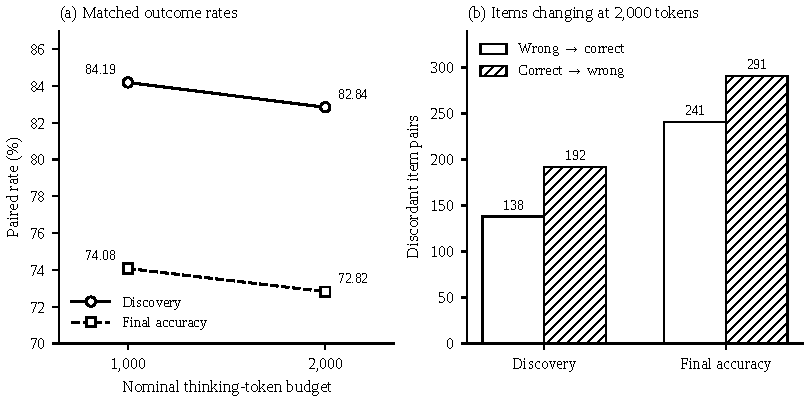
\includegraphics[width=0.92\textwidth]{figures/budget_tradeoff.pdf}
  \caption[Matched budget outcomes]{Matched aggregate outcomes at 1,000 and 2,000 nominal thinking tokens. The larger budget increases mean wall time while reducing machine-screened discovery and final semantic accuracy.}
  \label{fig:budget}
\end{figure}

The architecture-level results are heterogeneous. Debate final accuracy changes from 0.8113 to 0.7850 ($p=0.106$), Ensemble from 0.7725 to 0.7500 ($p=0.066$), Parallel Roles from 0.7425 to 0.7412 ($p=1.000$), Sequential from 0.6650 to 0.6538 ($p=0.426$), and Subtask Parallel from 0.7125 to 0.7113 ($p=1.000$). None of these individual final-accuracy comparisons reaches the conventional 0.05 level. The aggregate decline is produced by many small, mostly non-improving changes across cells rather than one architecture collapsing.

Latency increases in every system. Debate mean wall time rises from 15.38 to 22.92 seconds; Ensemble from 7.57 to 10.88; Parallel Roles from 9.94 to 14.79; Sequential from 17.89 to 22.58; and Subtask Parallel from 11.66 to 15.40. Parallel systems have shorter critical paths, but this should not be confused with lower total device work.

\section{Chapter summary}

The outcome experiments establish three constraints on the explanation developed in the following chapters. First, SAS is not universally superior: the ordering changes by dataset and architecture. Second, the completed fine-tuning intervention does not consistently remove the observed gaps. Third, a larger nominal token cap increases resource use without improving aggregate semantic outcomes. These findings motivate the next question: whether the systems fail because they do not discover a correct answer or because later components do not preserve it. \Cref{chap:machine-results} addresses that question using the full-trace machine screen.

\chapter{Machine-Screened Failure Analysis}
\label{chap:machine-results}

The benchmark results in \Cref{chap:benchmark-results} establish final performance but do not identify the stage at which correctness appears or disappears. This chapter uses the frozen Mistral screening snapshot to analyse all 8,000 MAS item-configurations and 26,873 intermediate stage outputs. The results provide breadth and failure localisation; they are screening evidence rather than human-validated prevalence estimates.

\section{Semantic discovery, oracle coverage, and aggregation regret}

The full-trace Mistral screen indicates that independent-candidate architectures frequently make the correct answer available before the final decision. Aggregation regret, defined in \Cref{eq:regret} as candidate-oracle accuracy minus final semantic accuracy, is the quantity that separates the two. For frozen MuSiQue at 1,000 tokens, Debate has final semantic accuracy 0.720 and candidate-oracle accuracy 0.845, giving aggregation regret of 0.125. Ensemble has final accuracy 0.660 and oracle accuracy 0.960, a regret of 0.300. Parallel Roles is more extreme: final accuracy 0.600 versus oracle accuracy 0.915, a regret of 0.315. These gaps are too large to describe as candidate-generation failure alone.

\begin{figure}[htbp]
  \centering
  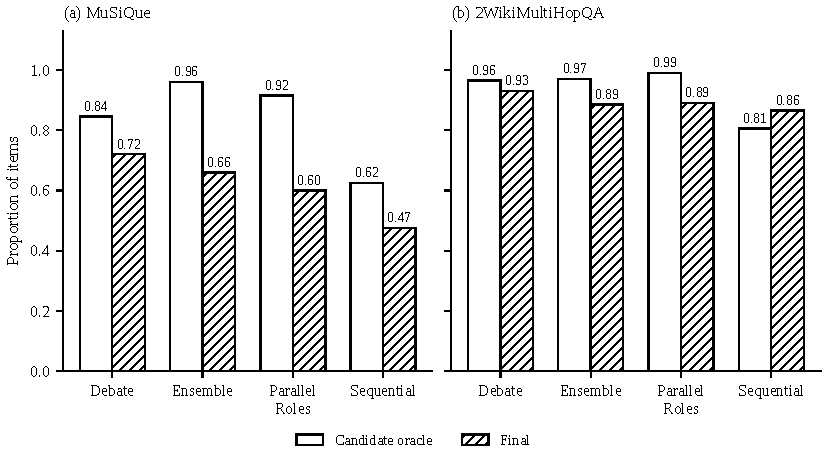
\includegraphics[width=0.94\textwidth]{figures/semantic_oracle_final.pdf}
  \caption[Candidate-oracle and final semantic accuracy]{Machine-screened candidate-oracle and final semantic accuracy for the frozen model at the 1,000-token budget. Higher oracle than final accuracy indicates that a correct candidate was available but not selected. Subtask Parallel is omitted because its worker outputs are partial findings rather than full-answer candidates.}
  \label{fig:oracle-final}
\end{figure}

\Cref{fig:oracle-final} shows that the gap is dataset dependent. On frozen 2Wiki at 1,000 tokens, Debate's final accuracy is 0.930 and its oracle accuracy 0.965, a regret of only 0.035. Ensemble and Parallel Roles still show positive regret, at 0.085 and 0.100. Easier questions allow both candidates and aggregators to be more reliable; on MuSiQue, candidate diversity increases without a comparable increase in final decision quality.

The semantic diversity statistic supports this interpretation. Frozen MuSiQue Parallel Roles has diversity rate 0.650 and a mean of four distinct candidate texts, while its final semantic accuracy is only 0.600. Ensemble has mean 3.835 distinct candidates and final accuracy 0.660. Diversity is therefore a resource, not an outcome. It creates selection opportunities and selection risk simultaneously.

Sequential behaves differently. In this machine-screened breadth analysis, its candidate oracle is an any-correct summary over the worker outputs, whereas the human final-boundary audit uses only the last worker as its source. These quantities must not be conflated. On frozen MuSiQue at 1,000 tokens, the worker-set oracle is 0.625 and final accuracy is 0.475. On 2Wiki, final accuracy exceeds the worker-set oracle (0.865 versus 0.805 at 1,000), producing negative regret. This is consistent with an aggregator synthesising partial or implicit findings into a correct final response. Negative regret does not imply perfect preservation; it indicates that the final stage sometimes creates answer-equivalent content not credited in any individual worker output.

\section{Machine-screened terminal-failure attribution}

Across 8,000 MAS item-configurations, the rule-based screen classifies 5,876 trajectories as finally correct under the machine label and 2,124 as terminal failures (26.6\%). Of all configurations, 946 (11.8\%) end wrong with no correct intermediate Discovery detected; the implementation assigns these directly to the initial/proposal category rather than locating a first causal error step. Among the remaining terminal failures, 73 (0.9\%) are assigned to Debate revision, 75 (0.9\%) to the Sequential worker chain, 173 (2.2\%) to the Debate final picker, and 857 (10.7\%) to final aggregation. The last category includes Ensemble, Parallel Roles, Sequential, and Subtask Parallel and is the largest pooled assigned boundary class.

\begin{table}[htbp]
  \centering
  \caption[Machine-screened terminal-failure attribution]{Mutually exclusive rule-based terminal-failure classes as count (percentage of the architecture's 1,600 item-configurations). ``No detected discovery'' means that the final output is wrong and no correct intermediate Discovery was detected; it is not a stepwise localisation of the first causal error. The final row uses all 8,000 MAS item-configurations. These are descriptive screening estimates, not human-validated prevalence.}
  \label{tab:first-error}
  \scriptsize
  \setlength{\tabcolsep}{2.5pt}
  \begin{tabular}{@{}lrrrrrr@{}}
    \toprule
    System & \shortstack{No detected\\discovery} & Revision & Worker chain & Picker & Aggregator & \shortstack{Any terminal\\failure} \\
    \midrule
    Debate & 77 (4.8) & 73 (4.6) & 0 (0.0) & 173 (10.8) & 0 (0.0) & 323 (20.2) \\
    Ensemble & 66 (4.1) & 0 (0.0) & 0 (0.0) & 0 (0.0) & 316 (19.8) & 382 (23.9) \\
    Parallel Roles & 77 (4.8) & 0 (0.0) & 0 (0.0) & 0 (0.0) & 336 (21.0) & 413 (25.8) \\
    Sequential & 376 (23.5) & 0 (0.0) & 75 (4.7) & 0 (0.0) & 94 (5.9) & 545 (34.1) \\
    Subtask Parallel & 350 (21.9) & 0 (0.0) & 0 (0.0) & 0 (0.0) & 111 (6.9) & 461 (28.8) \\
    \midrule
    All & 946 (11.8) & 73 (0.9) & 75 (0.9) & 173 (2.2) & 857 (10.7) & 2,124 (26.6) \\
    \bottomrule
  \end{tabular}
\end{table}

These rates make the architecture denominators explicit: for example, Sequential's 94 aggregator losses are 5.9\% of its 1,600 screened item-configurations, whereas Ensemble's 316 aggregation failures are 19.8\%. They should not be compared with a supposed SAS ``aggregation rate'': SAS has no picker or aggregator, and the same Mistral pre-final-Discovery-to-final-Endorsement screen has not yet been completed for its 1,600 traces.

Within Debate, the screen counts 278 harmful proposal-to-revision flips and 169 beneficial flips. A targeted human sensitivity audit exactly confirmed 13 of 24 resolved sampled harmful flips and 11 of 25 beneficial flips. A descriptive projection retained the direction harmful greater than beneficial, but the modest confirmation rates mean the raw full-trace counts cannot be presented as exact semantic totals. Similarly, the machine screen identifies 142 Sequential items where the worker chain ends wrong after earlier discovery and 94 in which the aggregator loses a correct last-worker answer. Only 8 of 25 sampled machine-labelled Sequential \ctow{} transitions were exactly confirmed in the targeted audit, mainly because the judge over-called source correctness.

These results locate picker and aggregator boundaries as high-value targets, but they do not substitute for the final human audit.

\section{Resource associations and truncation}

Within matched design strata, observations above the median wall time have lower odds of discovery (adjusted OR 0.657, 95\% CI $[0.574,0.753]$) and higher odds of dropping the answer after discovery (OR 1.768, $[1.529,2.044]$). Above-median realised thinking tokens show the same direction: OR 0.529 ($[0.456,0.613]$) for discovery and OR 2.679 ($[2.153,3.334]$) for post-discovery drop.

\begin{figure}[htbp]
  \centering
  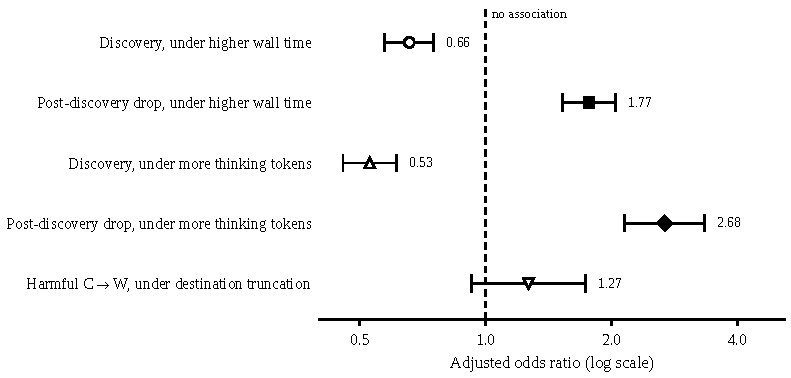
\includegraphics[width=0.90\textwidth]{figures/resource_associations.pdf}
  \caption[Resource exposure and semantic outcomes]{Adjusted observational odds ratios for resource exposure and semantic outcomes. Values below one favour the unexposed group for the named outcome; intervals are 95\% confidence intervals. These associations are not causal effects.}
  \label{fig:resources}
\end{figure}

These results do not mean that fewer tokens causally improve reasoning. Difficult or unstable items may elicit longer trajectories, and repeated unsuccessful revisions may consume both time and tokens. They show that realised compute is not a valid proxy for productive reasoning in this experiment.

Destination-stage truncation has OR 1.268 for a \ctow{} transition conditional on a correct machine-labelled source, with 95\% CI $[0.926,1.736]$ and $p=0.139$. The interval includes one, so the data do not establish a truncation effect. Furthermore, the targeted human audit found lower exact machine--human transition agreement for truncated destinations (0.412) than for non-truncated destinations (0.604). Truncation is thus both a plausible failure mechanism and a condition under which the automated judge is less dependable; the present evidence is insufficient to make a causal claim.

\section{Why human validation is required}

The broad screen supplies scale, but its most consequential errors occur in the transition-enriched cases required for mechanism claims. A single source-stage error can change an item's transition class, and the machine counts above therefore cannot be interpreted as exact failure prevalence. \Cref{chap:human-results} first evaluates audit reliability and then reports the population-weighted transition estimates derived from human labels.

\chapter{Human Audit and Transition Results}
\label{chap:human-results}

This chapter reports the controlling evidence for the final coordination boundary in Debate and Sequential. The audit contains 160 distinct item-configurations drawn from 160 distinct benchmark question identifiers: 80 Debate runs and 80 Sequential runs. These item-configurations produce 400 non-repeat stage records, and 20 blinded duplicate records are inserted only to measure intra-rater repeatability. The item-level dataset contains 15 named fields of mixed type; these are not 15 independent binary error labels.

\section{Human audit reliability}

The 20 hidden repeated stages produced exact agreement of 20/20 on both Discovery and Endorsement, with $\kappa=1.000$ and bootstrap intervals $[1.000,1.000]$. This shows perfect repeatability for the inserted records. It does not show independent inter-annotator validity because the same annotator labelled both blind copies.

Against the frozen Mistral stage labels, human agreement is 330/400 (82.5\%) for Discovery and 322/400 (80.5\%) for Endorsement. Cohen's kappa is 0.632 (95\% bootstrap CI $[0.557,0.705]$) for Discovery and 0.617 ($[0.541,0.691]$) for Endorsement. These values support use of Mistral for broad screening and sampling, but the 70 Discovery disagreements and 78 Endorsement disagreements are not negligible in a transition analysis.

\begin{table}[htbp]
  \centering
  \caption[Human audit reliability]{Human audit reliability. Human--machine agreement uses 400 non-repeat stage records; repeat agreement uses 20 hidden pairs.}
  \label{tab:agreement}
  \begin{tabular}{@{}llrrl@{}}
    \toprule
    Comparison & Axis & Exact agreement & $\kappa$ & 95\% CI \\
    \midrule
    Hidden repeat & Discovery & 20/20 (100.0\%) & 1.000 & [1.000, 1.000] \\
    Hidden repeat & Endorsement & 20/20 (100.0\%) & 1.000 & [1.000, 1.000] \\
    Human--Mistral & Discovery & 330/400 (82.5\%) & 0.632 & [0.557, 0.705] \\
    Human--Mistral & Endorsement & 322/400 (80.5\%) & 0.617 & [0.541, 0.691] \\
    \bottomrule
  \end{tabular}
\end{table}

Across all 420 annotation rows, the 14 cases with Discovery \correct{} and Endorsement \wrong{} demonstrate why a single semantic-correctness label is insufficient. The stage contains the answer but does not support the system selecting it. A presence-oriented judge is likely to over-credit precisely these cases.

\section{Human transition estimates}

The raw audited item transitions differ sharply by architecture. Debate contains 35 \correct$\rightarrow$\correct, 19 \ctow, zero \wtoc, 25 \wrong$\rightarrow$\wrong, and one \uncertain$\rightarrow$\wrong item. Sequential contains 40 \correct$\rightarrow$\correct, four \ctow, six \wtoc, 29 \wrong$\rightarrow$\wrong, and one \uncertain$\rightarrow$\wrong item. Because rare machine-defined transition strata were oversampled, the weighted rates rather than these raw proportions are used for population interpretation.

\begin{figure}[htbp]
  \centering
  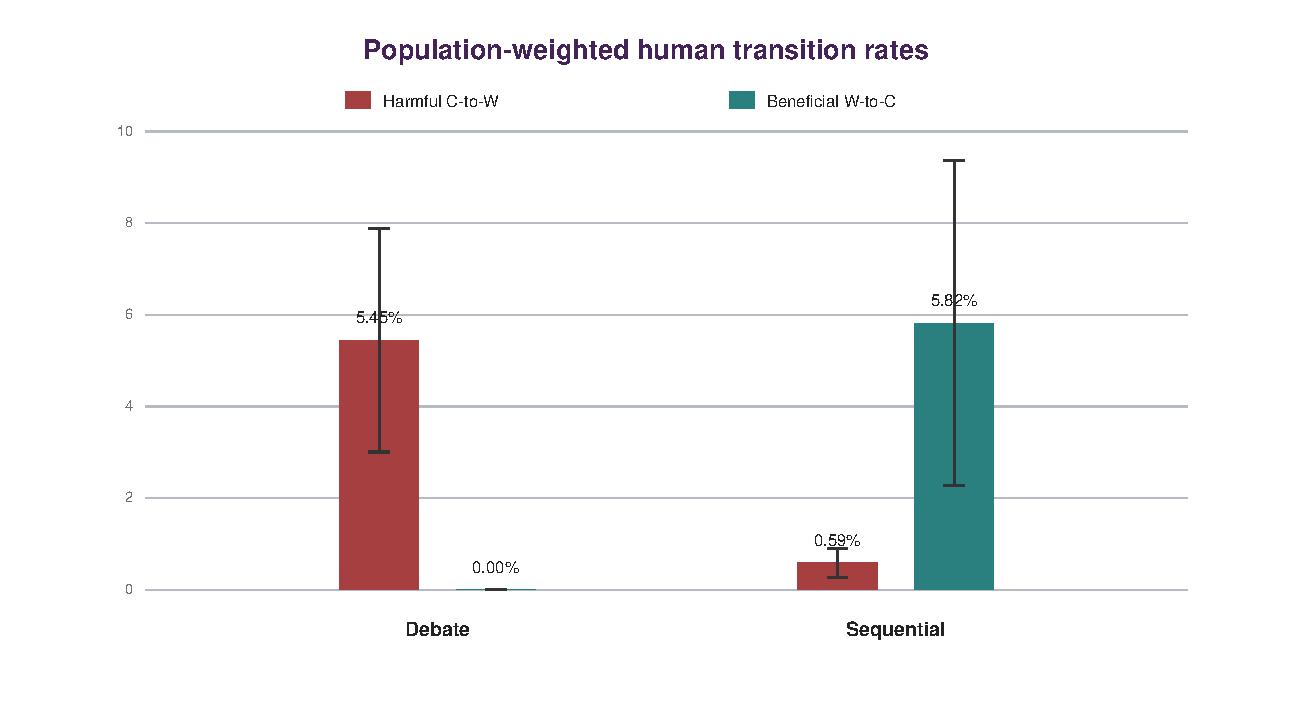
\includegraphics[width=0.88\textwidth]{figures/human_transition_rates.pdf}
  \caption[Population-weighted human transition rates]{Population-weighted human Endorsement transition rates under the primary \uncertain$\rightarrow$\wrong{} rule. Error bars are approximate 95\% finite-population stratified intervals.}
  \label{fig:human-transitions}
\end{figure}

Debate's weighted harmful \ctow{} rate is 5.45\% (approximate 95\% CI $[3.01,7.89]$), compared with 0.59\% for Sequential ($[0.27,0.90]$). The Debate-minus-Sequential difference is 4.86 percentage points ($[2.41,7.32]$). The beneficial \wtoc{} pattern is reversed: 0.00\% for Debate and 5.82\% for Sequential ($[2.28,9.37]$). The one machine-defined Debate beneficial picker event in the sampling census was human \correct$\rightarrow$\correct after unblinding, so no audited Debate wrong source was corrected by the picker.

Using source Discovery rather than source Endorsement gives a weighted probability that a discovered answer is not endorsed in the final output of 7.06\% for Debate and 3.96\% for Sequential. This second measure captures loss between informational presence and decision, including cases where a correct answer was discovered without being cleanly endorsed at the source.

\section{Sensitivity to uncertain labels}

The uncertain-label sensitivity analysis does not reverse the main harmful-rate ordering. Under \uncertain$\rightarrow$\wrong, exclusion of uncertain-bearing items, and \uncertain$\rightarrow$\correct, Debate's harmful rate is 5.45\%, 5.51\%, and 6.58\%, while Sequential's is 0.59\%, 0.60\%, and 2.20\%. The absolute Sequential estimate is more sensitive because one uncertain case has greater influence in a low-rate architecture, but Debate remains higher under every rule.

\section{Scope of the human comparison}

The human transition audit supports a comparison of the final coordination boundaries in Debate and Sequential; it does not by itself explain why SAS outperforms a MAS in a particular benchmark condition. SAS remains part of the final-performance benchmark in \Cref{chap:benchmark-results}. A cross-architecture process comparison should apply the same machine-screening pipeline to SAS and use pre-final Discovery to final Endorsement as the common transition, because SAS has no equivalent multi-agent picker or aggregator. Unless that additional analysis is completed and reported, the dissertation should not claim that SAS wins because it experiences a lower human-audited transition rate.

\section{Chapter summary}

The human audit changes the scale of the machine-screened transition estimates but retains an architecture-specific asymmetry. The final Debate picker is a measurable loss point, whereas the Sequential aggregator is less often destructive and sometimes corrective. This conclusion is bounded to the audited source definitions and weighted sampling frames. It does not establish that Sequential is globally superior to Debate or that the same rates apply to the three other MAS architectures.

\chapter{Discussion}
\label{chap:discussion}

\section{The central finding: exploration and decision separate}

The results support a simple but consequential conclusion: producing a correct answer somewhere in a multi-agent trace is not the same as delivering it. Independent candidates increase the chance that useful content appears, especially for Ensemble and Parallel Roles, yet their oracle-final gaps show that a final language-model decision frequently fails to exploit that content. Debate provides the clearest audited instance. Its revised candidate set can contain a correctly endorsed answer, but the final picker loses that state at a weighted rate of 5.45\% and does not produce an audited beneficial wrong-to-correct transition. Sequential shows the opposite final-boundary pattern: destructive aggregation is rare and the aggregator sometimes repairs a wrong last-worker state.

This does not establish that Sequential is globally better than Debate. Sequential's upstream discovery is weaker, particularly on MuSiQue, and an aggregator cannot recover evidence that never enters the chain. Debate frequently achieves stronger final accuracy and high semantic discovery. The result is instead a decomposition of capability. Debate appears better at candidate generation but less reliable at final selection; Sequential has a weaker source state but a more constructive final aggregator. Architecture choice should therefore depend on which component is limiting performance.

The distinction also clarifies why final accuracy can mask design problems. A Debate system may finish correctly even after a harmful revision if the other candidate remains correct. A Sequential aggregator may finish correctly despite a wrong last worker by synthesising earlier findings. Conversely, a system may have high discovery and low final accuracy. Transition analysis exposes these compensating pathways rather than assigning all credit or blame to the architecture as a whole.

\section{Why Debate can lose correct answers}

Debate assumes that exposure to an alternative argument helps an agent revise errors and helps a picker choose the better position. The machine screen suggests both beneficial and harmful revisions, but the targeted audit shows that the judge substantially overstates some of these transitions. The final human audit nevertheless provides strong evidence that the picker is not reliably corrective in the sampled population.

Several mechanisms are plausible. First, revised outputs can converge linguistically even when evidence remains asymmetric. A confident wrong answer may supply a clean narrative that is easier for the picker to recognise than a correct but qualified answer. Second, the picker receives model-generated summaries rather than a protected evidence graph. It may evaluate rhetorical coherence instead of entailment from the oracle context. Third, agents share the same model family and prompts, so their errors are not independent. Debate between correlated agents can amplify a shared shortcut rather than supply genuine epistemic diversity. Finally, the picker is a further generative call with its own exposure to truncation, extraction, and formatting errors.

These mechanisms should be treated as interpretations rather than directly identified causes. The audit labels correctness transitions, not latent persuasion. However, they lead to concrete design tests. A picker could be required to cite the exact evidence span supporting its choice. Candidate identities and confidence could be hidden to reduce stylistic bias. The system could preserve all answer-bearing claims in a structured table before revision. A deterministic evidence-based selector could also be compared against the generative picker. Each intervention targets selection without changing candidate generation, allowing the oracle-final gap to be tested directly.

\section{Why Sequential aggregation can recover}

Sequential's beneficial final transitions indicate that a wrong last-worker endorsement does not necessarily mean the accumulated trace lacks the answer. The aggregator sees the plan and worker history and may combine a correct earlier finding with the final subproblem result. In that sense it operates as a synthesiser rather than a simple selector. This explains why Sequential final semantic accuracy can exceed the designated candidate-oracle measure on some 2Wiki cells.

The architecture still has serious upstream weaknesses. Workers are serially dependent, later prompts contain growing context, and a final worker may focus on its assigned relation rather than restating the full answer. The machine screen's worker-chain losses and relatively low discovery rate suggest that relevant evidence can disappear before aggregation. The appropriate intervention is therefore different from Debate. Sequential systems need explicit state persistence: a structured ledger of established entities and relations, provenance for each intermediate fact, and constraints that prevent later workers from replacing validated findings without contrary evidence.

The beneficial aggregator result also cautions against judging intermediate workers by final-answer criteria alone. A worker assigned one hop may be correct and useful without endorsing the complete gold answer. Discovery and Endorsement labels help, but role-aware utility labels would be an even better future measure for partial subtask outputs.

\section{More computation is not necessarily more reasoning}

Doubling the nominal budget produces the expected resource increase but not an accuracy increase. Aggregate discovery and final semantic accuracy both decline, with more correct-to-wrong than wrong-to-correct paired changes. The pooled McNemar results are exploratory because they do not adjust for repeated appearances of the same question across conditions, but the descriptive direction is consistent across the aggregate counts and no architecture-level final-accuracy comparison shows a conventional 0.05-level improvement. This pattern is consistent with the argument that matched or greater token budgets do not guarantee an MAS advantage \citep{tran2026single}. It also shows where additional work can be unproductive in this dataset: longer trajectories are associated with lower discovery and greater post-discovery loss.

Three explanations are compatible with the data. First, additional tokens may be spent repeating context or generating stylistic elaboration rather than new evidence. Second, a longer allowance creates more opportunities for revision drift: a model can reason past a correct concise answer into a speculative alternative. Third, realised token use is endogenous. Hard questions and unstable states may naturally consume more tokens, so the association between longer output and error can arise without tokens causing the error. The paired cap experiment provides stronger evidence that the larger allowance did not help aggregate performance, but it still does not identify which of these mechanisms dominates.

The practical implication is to allocate compute conditionally. A system should stop when evidence and answer endorsement are stable, and spend additional budget only when candidate disagreement or missing hops justify it. Confidence alone may be poorly calibrated, so stopping should use observable conditions: agreement on an evidence-backed entity, complete coverage of plan steps, and absence of unresolved contradictions. This is more defensible than treating a maximum token count as a target.

\section{Implications for evaluation}

The project demonstrates why an evaluator needs both scale and auditability. The Mistral judge is useful: it processes tens of thousands of stages, highlights candidate failure points, and guides a focused human sample. Its broad stage agreement around 80\% is sufficient for exploratory summaries. It is not sufficient for declaring exact transition prevalence, especially when errors concentrate in the source state and when the target claim depends on rare flips.

The targeted calibration failure is itself a methodological result. A general validation set can be misleading when the downstream analysis conditions on hard cases selected by the same judge. This resembles spectrum bias: evaluator performance changes with the composition of the evaluated population. Future LLM-as-judge studies should validate on the strata used for substantive inference, not only on an overall random set. For transition analysis, validation should be pair-level because the derived class depends on both labels.

Separating Discovery from Endorsement also improves construct clarity. A single ``semantic correctness'' label can count an answer mention as success even when the stage rejects it. The audit found 14 such Discovery-correct, Endorsement-wrong rows. This is a small fraction of all annotations but directly concentrated in the mechanism of interest. An evaluator optimised for ordinary final answers may therefore fail exactly where debate and aggregation need to be studied.

\section{Implications for system design}

The results suggest four design principles.

\begin{enumerate}[leftmargin=*]
  \item \textbf{Protect discovered evidence.} Once a stage supplies an evidence-grounded candidate, store the claim and supporting span in a persistent structure. Later agents may challenge it, but should not silently erase it.
  \item \textbf{Separate generation from selection.} A selector should be evaluated independently on frozen candidate sets. Candidate coverage and picker accuracy answer different questions and should be optimised separately.
  \item \textbf{Use architecture-specific supervision.} Debate revision requires training on evidence-sensitive disagreement, while Sequential requires state tracking and synthesis. Generic instruction tuning may improve one component while leaving another unchanged.
  \item \textbf{Allocate compute adaptively.} Additional agents or tokens should be triggered by missing evidence or unresolved disagreement, not used uniformly. Stable answers with clear evidence should terminate early.
\end{enumerate}

The project's completed \texttt{v3b} checkpoint is largely aligned to single-agent behaviour. A natural extension is role-conditioned SFT using successful planner, worker, and aggregator traces. LoRA makes this feasible at modest training cost \citep{hu2021lora}, while Optima offers a related generate-filter-train perspective for multi-agent optimisation \citep{chen2024optima}. Such training must be evaluated with held-out traces and the same preservation metrics. Otherwise, an apparent gain in Sequential could be purchased by degrading the SAS or by teaching outputs that exploit the evaluator.

\section{Relationship to prior findings}

The findings neither wholly confirm nor reject prior debate research. \citet{du2023debate} and \citet{liang2023mad} demonstrate settings in which multi-agent interaction improves outcomes. The current 2Wiki results also include MAS gains, showing that the mechanism can work. The matched-budget MuSiQue results and the observed selection losses qualify the generality of that advantage. Model scale, task difficulty, candidate independence, and selector strength all matter.

The results align more directly with \citet{tran2026single}: once thinking budgets are controlled, a coherent single-agent trajectory remains a strong baseline and extra calls are not automatically productive. Building on that paper's theoretical, context-degradation, and qualitative failure accounts, this dissertation contributes an operational decomposition for the present setting: some MAS traces make answer-equivalent content available and then lose it at a measured final boundary. Communication quality and aggregation fidelity are therefore central variables in a compute-matched comparison, without implying that this is the only explanation for the observed performance gaps.

The work also extends self-consistency research \citep{wang2023selfconsistency}. Multiple samples can increase coverage, but the method of aggregation determines whether that coverage translates into accuracy. A learned generative aggregator is more flexible than majority voting but also less transparent. Reporting oracle accuracy, diversity, and regret alongside final accuracy makes this trade-off visible.

\section{Recommended next experiment}

The highest-value next experiment is a controlled selector replacement. Freeze the existing Debate revised candidates and compare three final decisions: the current generative picker, deterministic evidence matching against the oracle context, and a human selection. Because candidate generation remains identical, differences estimate selector quality without confounding from new proposals. The primary outcome should be human-audited \ctow{} and \wtoc{} rates, supplemented by final normalised accuracy and latency.

For Sequential, the corresponding experiment is a structured evidence ledger. Workers write entities, relations, and citations into immutable fields while retaining a free-text explanation. The final aggregator receives both the ledger and the transcript. A factorial ablation can test transcript only, ledger only, and both. This directly evaluates whether state persistence reduces worker-chain loss and whether the aggregator's beneficial transitions are maintained.

These experiments are preferable to immediately scaling the model or increasing the number of agents. They target the failure boundaries already identified and can reveal whether the architecture, rather than base capability, is the limiting factor.

\chapter{Limitations}
\label{chap:limitations}

\section{Model and task scope}

The main results use one 4-billion-parameter model family in frozen and project-fine-tuned forms. They do not establish that the same transition rates hold for larger proprietary models, mixture-of-experts systems, or models independently trained for each role. Shared-model agents may have unusually correlated errors. Conversely, a stronger selector might reduce aggregation regret even if candidate generation remains unchanged.

Only MuSiQue and 2WikiMultiHopQA are evaluated, both with oracle context. The design isolates reasoning and coordination but omits retrieval errors, tool use, long-horizon planning, and interactive environments. Multi-agent systems may offer different benefits when agents access genuinely different tools or information sources. The 200-item fixed validation subsets also limit precision for small architecture-by-dataset effects.

\section{Fine-tuning scope}

The \texttt{v3b} checkpoint is not a complete multi-agent training intervention. Its supervised data primarily preserve single-agent reasoning behaviour, so comparisons cannot answer whether role-specific training would make coordination reliably beneficial. Later role-conditioned \texttt{v4} plans and ratio arms were not included because they were not part of the completed, audited result set. Excluding them avoids presenting unfinished work as evidence but leaves the training question open.

\section{Semantic judge validity}

The Mistral judge does not meet the required reliability for exact transition inference. General calibration performance was strong, but targeted transition agreement fell to 73.9\% at the stage level and 50.5\% at the pair level. The full-trace terminal-failure attribution, semantic oracle values, and resource associations therefore remain machine-screened estimates. They are useful for pattern discovery and prioritisation, not ground truth.

The stronger Qwen2.5-72B judge also failed the later targeted acceptance rule detailed in \Cref{sec:calibration}. This rule is distinct from the earlier Discovery calibration, for which no numerical pass threshold had been preregistered. The result limits claims about all 26,873 stages and prevents a fully human-validated comparison of every architecture. A larger stratified audit, particularly for Ensemble and Parallel Roles aggregation, would be needed to confirm that their machine-estimated oracle-final gaps reflect the same mechanisms.

\section{Human audit limitations}

The final audit uses one annotator. Perfect hidden-repeat agreement demonstrates internal consistency for 20 duplicated stages but not inter-annotator reliability or freedom from systematic bias. The codebook and evidence verification reduce ambiguity, yet an independent second annotator and adjudication process would strengthen validity.

The audit sample is enriched for machine-defined transition strata and balanced greedily within strata. Population weights correct the deliberate oversampling at the stratum level, but the approximate confidence intervals assume more random sampling than the full selection procedure provides. The intervals should be read as descriptive uncertainty. Human--machine kappa intervals additionally resample stage records even though an item contributes multiple stages, so they do not adjust for within-item dependence. The weighted point estimates apply to the frozen audit population and should not be generalised beyond it without replication.

Only the final Debate and Sequential boundaries receive the primary human audit. Proposal-to-revision changes, earlier Sequential workers, and the final aggregators of other architectures are not equivalently validated. The dissertation is therefore strongest when stating that the audited Debate picker loses correct endorsements more often than the Sequential aggregator, and weaker when assigning exact prevalence to upstream machine-labelled failures.

\section{Compute measurement}

Thinking-token budgets are nominal caps, not perfectly equal total compute. Architectures differ in prompt length, number of calls, parallel execution, and uncounted generation overhead. Wall time for parallel systems reflects the critical path, not total GPU-seconds. Scheduler telemetry and power measurements would be required for a full cost or energy analysis.

Actual token use and wall time are endogenous to the trajectory. The adjusted odds ratios cannot show that longer reasoning causes lower discovery or greater loss. The paired budget intervention provides more credible evidence that the larger cap did not help aggregate outcomes, but even that comparison mixes the effects of additional available reasoning, changed truncation, and altered stopping behaviour. Its pooled McNemar tests also treat repeated condition-level observations from the same benchmark question as independent; without a question-clustered sensitivity analysis, the pooled $p$-values remain exploratory.

\section{Metric limitations}

Lexical accuracy can under-credit valid paraphrases and over-credit fortunate strings, and the two failures fall on opposite sides of the rule that is chosen. The headline benchmark metric is normalised containment (\Cref{eq:containment}), which credits any output in which an accepted answer string appears, including one that mentions the answer and then rejects it, but can miss a valid equivalent absent from the finite reference set. It is therefore a lexical outcome measure rather than a calibrated upper or lower bound on semantic correctness. Normalised exact match has a strong format bias, scoring a substantively correct sentence as wrong whenever the answer is embedded in explanatory text, which for Debate means an accuracy of 0.030 against 0.510 under containment on frozen MuSiQue at 1,000 tokens (\Cref{tab:metric-sensitivity}). Neither rule is a satisfactory measure of final-answer correctness on its own, which is why both are reported and why the substantive claims rest on the semantic and human layers rather than on either lexical figure. Semantic Discovery and Endorsement improve interpretability but remain discrete abstractions of rich text. Candidate-oracle accuracy also assumes that a correct candidate is usable by an ideal selector, which may be false if the output contains contradictory claims or insufficient provenance. For Subtask Parallel, partial findings make oracle comparisons particularly difficult.

Finally, this dissertation analyses observable output states rather than latent reasoning. It cannot prove that a model composed the intended evidence chain or that a correct answer was reached for the right reason. Evidence-grounded human labels reduce this risk but do not eliminate shortcut reasoning identified in prior work \citep{min2019compositional}.

\chapter{Conclusion}
\label{chap:conclusion}

This dissertation asked whether multi-agent language-model systems improve multi-hop question answering under matched thinking-token budgets and, more importantly, what happens after a correct answer first appears. The answer is not captured by a single global MAS-versus-SAS score. Architecture, dataset, and decision boundary all matter.

For RQ1, the benchmark shows that multi-agent decomposition can increase candidate discovery and can outperform the single-agent baseline in particular cells, such as frozen Debate on 2WikiMultiHopQA. It does not provide a consistent advantage. On MuSiQue, the SAS remains highly competitive, while Ensemble and Parallel Roles exhibit large machine-screened gaps between candidate-oracle and final accuracy. Candidate generation is therefore only one half of successful collaborative reasoning.

For RQ2, the blind human audit supplies the central result. Debate's final picker converts a correct source endorsement to a wrong final endorsement at a weighted rate of 5.45\%, compared with 0.59\% for the Sequential aggregator. The weighted harmful-rate difference is 4.86 percentage points. Beneficial wrong-to-correct transitions are 0.00\% for Debate and 5.82\% for Sequential. The finding is robust to all three treatments of uncertain labels. Debate is stronger at making candidate answers available, but its final selector is a measurable loss point; Sequential's final aggregator is less destructive and sometimes corrective.

For RQ3, doubling the nominal thinking budget raises mean wall time by 4.83 seconds per item while reducing aggregate semantic discovery from 84.19\% to 82.84\% and final semantic accuracy from 74.08\% to 72.82\%. More available computation is not equivalent to more useful reasoning. Longer trajectories can repeat, drift, and create additional opportunities to discard an already correct state.

The methodological conclusion is equally important. A broad calibration score for an LLM judge did not transfer to transition-enriched cases. Machine labels remain valuable for screening thousands of stages, but the primary transition claims require the human audit. Separating Discovery from Endorsement, validating at the pair level, and weighting frozen strata make the resulting claim more modest but more defensible.

The practical direction is to build systems that preserve evidence before adding more agents. Debate needs evidence-aware selection over frozen candidates. Sequential needs persistent structured state across workers. Both need adaptive stopping rather than uniform budget expansion. Multi-agent reasoning should be judged not by how many voices it creates, but by whether its coordination mechanisms reliably convert discovered evidence into the answer it finally endorses.


\appendix
\chapter{Human Audit Codebook Summary}
\label{app:codebook}

\section{Blind record fields}

Each annotation record contained a blind record identifier, question, accepted answer and aliases, supplied evidence, stage role, stage text, and completion status. Architecture, machine transition class, source run, sampling weight, and repeat identity were concealed until unblinding.

\section{Discovery rules}

\begin{longtable}{@{}p{0.15\textwidth}p{0.78\textwidth}@{}}
\toprule
Label & Operational rule \\
\midrule
\endhead
\correct & The stage contains the accepted answer, an accepted alias, or an evidence-grounded answer-equivalent relation sufficient to identify it. Mere string overlap without the required relation is insufficient. \\
\wrong & The answer-equivalent content is absent, points to a different entity or relation, or is only a contentless option reference. \\
\uncertain & The evidence and stage text do not permit a defensible label, normally because truncation interrupts the answer-bearing claim. \\
\bottomrule
\end{longtable}

\section{Endorsement rules}

\begin{longtable}{@{}p{0.15\textwidth}p{0.78\textwidth}@{}}
\toprule
Label & Operational rule \\
\midrule
\endhead
\correct & The stage's answer-bearing conclusion commits to the accepted answer or an answer-equivalent statement. \\
\wrong & The stage commits to a different answer, rejects the accepted answer, or never endorses answer-equivalent content. Mentioning the accepted answer as an unselected possibility remains wrong. \\
\uncertain & The commitment cannot be recovered because the answer-bearing statement is incomplete or truncated. \\
\bottomrule
\end{longtable}

\section{Primary audit counts}

The audit contains 160 unique items, 400 non-repeat stage records, and 20 hidden repeats. The 80 Debate items contain 35 \correct$\rightarrow$\correct, 19 \ctow, zero \wtoc, 25 \wrong$\rightarrow$\wrong, and one \uncertain$\rightarrow$\wrong transition. The 80 Sequential items contain 40 \correct$\rightarrow$\correct, four \ctow, six \wtoc, 29 \wrong$\rightarrow$\wrong, and one \uncertain$\rightarrow$\wrong transition. These raw counts must not be used as population rates because the sample deliberately oversamples machine-defined transition strata.

Reason-code harmonisation after unblinding changed three explanatory codes only. No C/W/U label, agreement statistic, or transition estimate changed.

\chapter{Reproducibility and Evidence Map}
\label{app:reproducibility}

\section{Core configurations}

The frozen and fine-tuned all-architecture token benchmarks are configured in:
\begin{itemize}[leftmargin=*]
  \item \path{configs/frozen_all_mas_token.yaml}
  \item \path{configs/v3b_all_mas_token.yaml}
  \item \path{configs/2wiki_frozen_token.yaml}
  \item \path{configs/2wiki_v3b_token.yaml}
\end{itemize}

Each records seed, decoding settings, model path, context mode, evaluation size, systems, architecture limits, and budget levels. The corresponding wall-clock configurations preserve the architecture definitions while changing the budget mode.

\section{Figure generation}

The figures are produced by two scripts in \path{dissertation/latex/}. \path{generate_figures.py} draws the two schematics (\Cref{fig:architecture-example} and \Cref{fig:pipeline}) with ReportLab. \path{generate_data_figures.py} draws the four data figures from the committed analysis CSV files using Matplotlib, together with the export and inspection helpers of the \emph{scientific-visualization} Agent Skill (K-Dense, MIT licence); set the \path{SCIVIZ_SKILL} environment variable to a checkout of that skill before running it. Each data figure is written with a companion \path{*.export.json} manifest recording its source file, the transformations applied, and how uncertainty is defined.

All figures are black on white. Series are separated by hatch pattern, marker shape and line style rather than by colour, so no information is lost in monochrome reproduction.

\section{Derived evidence files}

\begin{longtable}{@{}>{\raggedright\arraybackslash}p{0.38\textwidth}>{\raggedright\arraybackslash}p{0.55\textwidth}@{}}
\toprule
File & Role in the dissertation \\
\midrule
\endhead
\path{analysis/diagnostics/*/metrics.csv} & Lexical final accuracy, F1, candidate diversity, and preliminary stage diagnostics by run. \\
\path{analysis/semantic_diagnostics/semantic_metrics.csv} & Full-trace semantic discovery, oracle, final, preservation, regret, and architecture counters. \\
\path{analysis/semantic_diagnostics/first_error_stage.csv} & Machine-screened first terminal failure locations. \\
\path{analysis/semantic_diagnostics/budget_pair_tests.csv} & Matched 1,000-versus-2,000-token outcome tests and paired resource changes. \\
\path{analysis/semantic_diagnostics/budget_wallclock_overall.csv} & Architecture-level wall time, realised tokens, truncation, discovery, preservation, and final accuracy. \\
\path{analysis/semantic_diagnostics/resource_associations.csv} & Fixed-effect stratified resource and truncation odds ratios. \\
\path{analysis/cloud_revision_package/FROZEN_MISTRAL_SCREENING_PROMPT.md} & Readable frozen copy of the Mistral v4 system prompt, user-message template, model identifier, and inference settings. \\
\path{analysis/final_transition_endorsement_audit/blind_stage_review_400.csv} & Completed blind human labels for the 400 non-repeat records, with repeat material maintained in round files. \\
\path{analysis/final_transition_endorsement_audit/final_transition_audit_key.jsonl} & Frozen unblinding key joining record identifiers to architecture, item, role, and stratum. \\
\path{analysis/final_transition_endorsement_audit/unblind/item_level_unblinded_160.csv} & Item-level audit table containing the 15 documented truncation, human-state, human-transition, machine-state, and machine-transition fields used for the final boundary analysis. \\
\path{analysis/final_transition_endorsement_audit/UNBLIND_REPORT.md} & Agreement, weighted transition estimates, uncertainty sensitivity, and audit checks. \\
\path{analysis/final_transition_endorsement_audit/CODEBOOK_REV4.md} & Final decision rules used for Discovery and Endorsement. \\
\path{data/sft_train_v3.jsonl.stats.json} & Frozen v3b data-construction counts, coverage, sampling settings, and reasoning-length summary. \\
\path{src/build_sft_data_v3.py}, \path{src/train_lora_v3.py}, \path{src/merge_lora_v3.py} & Executable v3b rejection-sampling, completion-only LoRA training, and merge procedures. \\
\path{src/repair_final_audit_truncation_metadata.py} & Verified repair that restores unavailable final-stage truncation values to NA and recomputes the tri-state union without changing labels. \\
\bottomrule
\end{longtable}

\section{Reproduction sequence}

The analysis can be reproduced in five stages. First, run the fixed benchmark configurations and retain complete stage traces. Second, apply lexical scoring and deterministic alias normalisation. Third, generate the semantic screen with the frozen judge prompt and retain uncertain outputs rather than coercing them. Fourth, reconstruct the frozen audit strata and join the completed blind sheet only after annotation. Fifth, compute weighted transitions under the three uncertain-label rules and regenerate the tables and figures.

The supplied LaTeX project contains a figure-generation script that reads the committed CSV summaries and writes vector PDF figures. Running that script does not re-judge any model output and therefore cannot change semantic labels.

The final 160-item output tables are committed, but this package does not contain a standalone provenance script for the complete final unblinding and weighted-summary derivation. The earlier 100-pair sensitivity script must not be described as though it generated those tables. The narrow truncation-metadata repair listed above is independently asserted against the frozen audit key; it does not reconstruct or alter the human labels, strata, weights, or transition estimates.

\section{Scope exclusions}

Exploratory role-conditioned \texttt{v4} training plans, incomplete ratio arms, and any post-audit prompt experimentation are excluded from the main evidence. They remain potential future work but should not be mixed with the frozen benchmark and audit when reproducing the reported claims.


\backmatter
\bibliographystyle{plainnat}
\bibliography{references}

\end{document}
